
\documentclass[submit]{ipsj}
%\documentclass{ipsj}

\usepackage[dvipdfmx]{graphicx,xcolor}
\usepackage[fleqn]{amsmath}
\usepackage{newtxtext}
\usepackage{latexsym}
\usepackage[varg]{newtxmath}
\usepackage{multirow}
\usepackage{url}
\usepackage{booktabs}
\usepackage{tascmac}

\newcommand{\todo}[1]{\colorbox{yellow}{{\bf TODO}:}{\color{red} {\textbf{[#1]}}}}
\newcommand{\ihara}[1]{\colorbox{pink}{{\bf IHARA}:}{\color{blue} {\textbf{[#1]}}}}

\def\Underline{\setbox0\hbox\bgroup\let\\\endUnderline}
\def\endUnderline{\vphantom{y}\egroup\smash{\underline{\box0}}\\}
\def\|{\verb|}

\setcounter{巻数}{59}
\setcounter{号数}{1}
\setcounter{page}{1}


\受付{2025}{7}{\todo{最後}}
\採録{2025}{8}{\todo{最後}}




\begin{document}


\title{複数ソフトウェアの修正履歴の統合による\\コーディング規約違反の修正予測精度の評価}

\etitle{Evaluating the Prediction Accuracy of Coding Standard Violation Fixes through Integrated Software Change History Data}

\affiliate{WU}{和歌山大学\\
Wakayama University, 930 Sakaedani, Wakayama 640--8510, Japan}


% \paffiliate{WU}{和歌山大学\\
% Wakayama University}

\author{亀岡 令}{Ryo Kameoka}{WU}
\author{伊原 彰紀}{Akinori Ihara}{WU}

\begin{abstract}
ソフトウェア開発プロジェクトが,コーディングスタイルを共通化するために,独自で設定したコーディング規約に違反するソースコードを自動検出する静的解析ツールが頻繁に使用される.しかし,規約違反コード\todo{この言葉を頻繁に使うならこのままで良い.あまり使わないなら「規約するソースコード」に置き換え}を大量に検出するため,一部の規約違反コードのみが修正されることが多い.従来研究では,プロジェクトの修正履歴に基づき,機械学習を用いて修正すべき規約違反コードを推薦するモデル(\todo{規約違反コードの修正要否判定モデル?})を開発しているが,修正履歴に正例数(修正された違反コード)が少ない場合に予測精度が低いという課題があった.本研究では,他のプロジェクトの修正履歴も学習データに含める違反修正要否判定モデルを提案する.\todo{N件}のオープンソースプロジェクトを対象にケーススタディを実施した結果,\todo{どうだった?}
%OSS開発では,可読性の高いソースコードが重要であり,コーディング規約はそのための手段となる.しかし,規約違反コードは大量に検出されるため,修正は一部に留まることが多い.従来研究では,プロジェクト自身の修正履歴に基づき違反箇所の修正優先度を予測してきたが,予測精度が十分でない場合が多い.本研究では,他の複数プロジェクトの開発履歴を学習させることによる予測精度の変化を検証し,予測精度が向上する条件について分析する.
\end{abstract}


\begin{jkeyword}
静的解析, 機械学習, 可読性
\end{jkeyword}

\begin{eabstract}
\todo{未修正}In Open Source Software (OSS) development, highly readable source code is crucial, and coding standards serve as a means to achieve this. However, since a large number of coding standard violations are detected, only a fraction of them are often fixed. Conventional studies have predicted the fix priority of violation locations based on the project's own modification history, but the prediction accuracy has often been insufficient. This research investigates the change in prediction accuracy by training models with development histories from multiple other projects and analyzes the conditions under which prediction accuracy improves.
\end{eabstract}

\begin{ekeyword}
Static Analysis, Machine Learning, Readability
\end{ekeyword}

\maketitle

\section{はじめに}

コーディング規約は,ソースコードの記述方法に関する禁止事項や推奨事項を定め, 可読性や保守性を高めるためのコーディングスタイルの取り決めである.
ソフトウェア開発プロジェクトは,実装に参加する開発者にコーディングスタイルの共通化や, ソースコードの最適化のためにコーディング規約の遵守を促すことで, 可読性や保守性の高いソースコードを共有することができる\cite{EffectsSAT}. 具体的には,開発者にとってのソースコードの理解容易性や,バグの早期発見に貢献している\cite{Beller2}\cite{Johnson}\cite{Beller}.

%コーディング規約とは, ソースコードを一定の品質に保つための記述方法について, 禁止事項や推奨事項を定め, 保守性を高めるためのコーディングスタイルなどをまとめたものである. 
% ソフトウェア開発者はコーディングスタイルの共通化や, ソースコードの最適化のためにコーディング規約を遵守することで, 可読性の高いソースコードを書くことができる\cite{EffectsSAT}. 
% また, プロジェクトへのコーディング規約の導入によって, ソースコードの理解の促進やバグの早期発見などへの効果も確認されている\cite{Beller2}\cite{Johnson}\cite{Beller}.

コーディング規約に違反しているコード断片(\todo{以降,規約違反コード})を機械的に検出するために,多くのプロジェクトは静的解析ツールを使用している.
静的解析ツールは, ソースコード中の規約違反コードを正規表現などによりソースコードを実行することなく検出できるため, 継続的インテグレーションのプロセスの1つとして使用されることも多い.\todo{プログラミング言語ごとに規約違反のテンプレートを提供していると書いても良さそう}プログラミング言語別に提供される規約違反のリストには,規約違反の種類を多数定義しているため,一部の違反のみ有効にしているプロジェクトも存在する\todo{引用?}しかし,開発者が有効に設定されたすべての規約違反を修正しておらず,従来研究による実証実験によると\todo{X\%}の規約違反コードは修正されていない.静的解析ツールが検出する膨大な規約違反コードの中から,修正を要する規約違反コードを分類することは開発効率の低下につながるため,修正が必要な規約違反コードを分類するための研究が行われている\cite{Nguyen}.

% コーディング規約に違反している箇所を機械的に検出するためには静的解析ツールが用いられる. 
% 静的解析ツールはソースコードを実行することなく, ソースコードに含まれるコーディング規約に違反している箇所を検出することができ, 継続的インテグレーションのプロセスの1つとして使用されることも多い. 
% 静的解析ツールは, ソースコード中のコーディング規約に違反しているコード断片を正規表現などにより検出することができるため, 開発者は静的解析ツールが検出した違反を確認することで, コーディング規約に違反している箇所を速やかに修正することができる. 
% 静的解析ツールは多くの規約の種類を定義しているため, 修正の必要がないような軽微な違反を含む大量の規約違反検出結果が出力されることが頻繁に発生する.
% 静的解析ツールの大量の検出結果は開発効率の低下につながるため, 修正が必要な違反を検出するための研究が行われている\cite{Nguyen}.



従来研究では,大量に検出される規約違反コードの中から修正すべき違反を検出する手法が数多く提案されている\cite{JyuraiPre}.静的解析ツールの検出結果を優先度づけする研究も数多く行われている.\todo{1文目と2文目で何が違う?大差ないなら1文にまとめ,「数多く」ならもう少し引用がほしいです.}
%従来研究の多くは, 評価対象プロジェクトの規約違反コードの修正履歴を学習モデル構築手法を提案している.予測精度が十分でない場合が多い. その原因の一つとして, 学習データのスパース性が考えられる. 学習データ数自体は十分でも正例数が少なく, 学習が十分できないことが考えられる. Tabassumらは, 不具合予測やソースコードの自動修正において, データ不足やコールドスタート問題への対応として, 異なるプロジェクトの開発データを用いることによって学習データを補う手法を提案しているが, 不具合予測であり, コーディング規約違反に関する研究は行われていない\cite{Tabassum}. 異なるプロジェクトのデータを用いることでコールドスタート問題への対処は可能であるが, 実装方針の異なるプロジェクトのデータを学習することとなるため, 十分なデータがある場合には, 単一プロジェクトのデータのみを学習したほうが高い予測精度を得られる可能性がある.
従来研究では、特定のプロジェクトにおいて,過去の規約違反コードの修正履歴を学習しモデルを構築する手法を提案している.当該手法は,学習データの総数は多くても正例が少ないプロジェクトで予測精度が低くなる課題を有する.Tabassumらは,不具合予測やソースコード自動修正の分野で,データ不足やコールドスタート問題に対応するため,異なるプロジェクトの開発履歴を利用して学習データを補う手法を提案している\cite{Tabassum}.規約違反コードの検出においても,異なるプロジェクトのデータを利用すれることでコールドスタート問題の解消が期待できる一方で,実装方針の異なるプロジェクトのデータを学習することで精度が低下する課題も考えられる.

% 従来研究では, 大量に検出される規約違反コードの中から修正すべき違反を検出する手法が数多く提案されている\cite{JyuraiPre}.静的解析ツールの検出結果を優先度づけする研究も数多く行われている. 従来研究の多くは, 単一プロジェクトの規約違反修正履歴を学習することで各プロジェクトのコーディングの慣習を捉えた予測を行っているが, 予測精度が十分でない場合が多い. その原因の一つとして, 学習データのスパース性が考えられる. 学習データ数自体は十分でも正例数が少なく, 学習が十分できないことが考えられる. Tabassumらは, 不具合予測やソースコードの自動修正において, データ不足やコールドスタート問題への対応として, 異なるプロジェクトの開発データを用いることによって学習データを補う手法を提案しているが, 不具合予測であり, コーディング規約違反に関する研究は行われていない\cite{Tabassum}. 異なるプロジェクトのデータを用いることでコールドスタート問題への対処は可能であるが, 実装方針の異なるプロジェクトのデータを学習することとなるため, 十分なデータがある場合には, 単一プロジェクトのデータのみを学習したほうが高い予測精度を得られる可能性がある.

本研究では,複数プロジェクトの開発履歴を予測モデルの学習に用いることによる規約違反コードの修正予測精度を明らかにする.提案手法として,2種類の予測モデルを構築する.1つは,複数プロジェクトの開発履歴を単純に結合して学習する手法である(全学習手法).もう1つは,\todo{XX}が類似する複数プロジェクトの開発履歴を結合して学習する手法である(選定学習).本研究の提案は、著者らが以前に提案した手法\cite{mine}\cite{mine_live}を拡張し,類似プロジェクトのみを統合する選定学習を新たに導入した点にある.評価の結果,一部のプロジェクトにおいて再現率が大幅に改善された.\todo{一部のように弱気に書くか悩みどころ.}

従来研究ではLLMを用いて修正要否を検出すると,修正の必要がない箇所まで変更されることが指摘されている\todo{輪講か何かで聞いたような?}.本研究の結果をLLMのファインチューニングに用いることで,修正すべき違反のみを検出し,修正することが期待される.

% 本研究では, 複数プロジェクトの開発データを予測モデルの学習に使用することによる, コーディング規約違反の修正予測精度への影響を明らかにする. 提案手法として2種類の予測モデルを構築する. 1つは, 複数プロジェクトのデータを単純に結合し学習する全学習手法である. もう1つは, 複数プロジェクトのデータを統合する際に, 類似するプロジェクトに絞り, 統合し学習する選定学習手法である. 本研究の提案手法は, 著者らが過去に提案した手法から, 類似したプロジェクトのみを学習データに統合する選定学習を新たに提案している\cite{mine}\cite{mine_live}. 選定学習の結果として, 一部プロジェクトにおいて, 再現率の大幅な改善が見られた.

% 本研究の貢献として, 静的解析ツールの結果から修正すべき違反のみを正確に推薦することができれば, 必要修正箇所のみをLLMなどを用いたコードの自動修正を行うことが可能となり, コードの品質を高く保つことが容易になる.

続く\ref{chap:background}章では, コーディング規約違反の検出と, 従来研究について述べる. \ref{chap:approach}章では本研究における実験の全体像と提案手法について述べる. \ref{chap:result}章では評価結果を示し, \ref{chap:consideration}章では考察を述べる. \ref{chap:heuristic}章では本研究の妥当性への脅威について述べ, \ref{chap:end}章でまとめる.



%%%%%%%%%%%%%%%%%%%%%%%%%%%%%%%%%%%%%%%
\section{コーディング規約と規約違反の検出}\label{chap:background}
%%%%%%%%%%%%%%%%%%%%%%%%%%%%%%%%%%%%%%%

\subsection{コーディング規約違反}

コーディング規約は,複数人によるソフトウェア開発においてソースコードの記述方法を共通化するための指針である.規約には,変数やクラスの命名規則,関数の長さや複雑度の上限といった可読性に関するルール,エラーの原因となる記述の検出,禁止事項,制限事項,推奨事項などが含まれる.
% コーディング規約は,オープンソースソフトウェア開発や開発チームのように複数人でソフトウェアを開発する際に,プログラミングにおける記述方法を標準化するための指針である.規約には,変数やクラスの命名規則,関数の長さや複雑度の上限といった可読性に関するルール,エラーの原因となる記述の検出,禁止事項,制限事項,推奨事項などが含まれる.
これらのコーディング規約は,プログラミング言語ごとに異なる内容や基準を持ち,複数の規約が存在する.例えば,Python言語にはPEP8,Java言語にはCode Conventions for the Java Programming LanguageやGoogle Java Style Guide,JavaScript言語にはGoogle JavaScript Style GuideやAirbnb JavaScript Style Guideなどがある.
開発者は,各プロジェクトが参照する規約,違反検出時の出力形式を調整を加えながら,静的解析ツールを用いて規約違反コードを検出している.プロジェクトの中には,継続的インテグレーション (CI) 環境に組み込むことで開発効率の向上を実現している\cite{ci/cd}.
%.静的解析ツールは言語ごとに複数存在し,参照する規約,違反検出時の出力形式,違反のカスタマイズ性などが異なる.開発者は,これらのツールを継続的インテグレーション(CI)環境に組み込むことで,開発効率の向上を図ることが可能である\cite{ci/cd}.
また,ソースコードの可読性や保守性といった品質を高水準で維持することは重要であり,品質の劣るコードには,良質なコードの約15倍の欠陥が含まれる可能性があることが報告されている\cite{静的解析ツールの効果}.\todo{これって静的解析ツールの効果?文章に静的解析ツールの話がないからわからない}

静的解析ツールは,ソースコード中の規約違反コードを網羅的に検出するが,その数は膨大であることが多く,開発者がそのすべてを確認,修正,保守するには多大なコストと労力を要する\cite{UsingStaticAnalysisTools2}.さらに,優先的に修正すべき違反を区別するためには,経験やソースコードへの深い理解が求められる\cite{shuseisarenai}.

%し,ユーザに提示する.しかし,この過程で検出される違反は膨大な数に上ることが多く,実際,先行研究では静的解析ツールが多数の規約違反を検出する傾向があることが指摘されている\cite{UsingStaticAnalysisTools2}.
% このような検出結果には,修正の優先度が低い軽微な違反も多数含まれており,開発者がすべてを確認・修正・保守するには多大なコストと労力を要する.さらに,どの違反を優先的に修正すべきかを判断するには,経験やソースコードへの深い理解が求められ,実用上の負担となっている\cite{shuseisarenai}.

\subsection{従来研究}


従来研究では,静的解析ツールによる大量に検出した規約違反コードの中から,機械学習を用いて修正すべき規約違反コードを分類する手法が提案されている\cite{JyuraiPre}\cite{beizu}.
Kimらは,静的解析ツールの出力をベイジアンネットワークに基づいて解析し,修正すべき規約違反コードを分類する手法を提案している\cite{beizu}.また,検出された違反に対する修正優先度付けする研究も数多く行われている\cite{Wang}\cite{Qing}\cite{HowFar}.これらの研究では,予測対象プロジェクトにおける規約違反の修正履歴を学習データとして用い,新たに検出された違反を評価対象とする機械学習モデル(規約違反コードの修正要否判定モデル)の構築と評価が行われている.



% 従来研究では,静的解析ツールによる大量の違反検出が開発効率の低下を招くことに対処するため,機械学習を用いて修正の優先度を予測する手法が提案されている.たとえば,Ruthruffらは,優先的に修正すべき違反を特定するための機械学習モデルを構築している\cite{JyuraiPre}.また,Kimらは,静的解析ツールの出力をベイジアンネットワークに基づいて解析し,違反の修正優先度を予測する手法を提案している\cite{beizu}.
% そのほかにも,検出された違反に対する修正優先度付けや修正要否の予測に関する研究が数多く行われている\cite{Wang}\cite{Qing}\cite{HowFar}.これらの研究では,予測対象プロジェクトにおける過去の規約違反修正履歴を学習データとし,新たに検出された違反を評価対象とすることで,予測モデルの構築と評価が行われている.

従来研究では,評価対象プロジェクトの修正履歴を学習データとして用いてモデルを構築している.これは各プロジェクトでコーディングスタイルや開発体制が異なり,評価対象と同一プロジェクトの修正履歴を学習することで高い精度が得られることが示されている.
% 従来研究では,一般に,評価対象プロジェクトの修正履歴を学習データとして用いて予測モデルを構築する.プロジェクトごとにコーディングスタイルや開発体制が異なるため,対象と同一プロジェクトの履歴を学習する方が,他プロジェクトの履歴を用いるよりも高い精度が得られると考えられている.
しかし,同一プロジェクトの学習データには,出現する違反の種類や修正率に偏りが生じることがある\cite{Panichella}\todo{この論文では予測まで行っていない?そのため,次の文であるように予測精度が低下する可能性,という表現になっているう?}.この結果,修正された違反(正例)と修正されなかった違反(負例)の数に不均衡が生じ,学習データが小規模となることで,予測精度の低下を招く可能性がある.

本研究では,評価対象以外のプロジェクトの修正履歴を学習データに含めることで,規約違反コードの修正予測精度の向上を目的とする.
%予測モデルの構築において,評価対象とは異なるプロジェクトのコーディング規約違反修正履歴を学習データとして用いることが,修正要否予測精度に与える影響を明らかにすることを目的とする.
従来研究では,名倉らが複数プロジェクトのデータを用いて規約違反の発生件数の増減を予測している.一方で,個々の規約違反コードの修正有無の予測は対象としていないため,本研究とは異なるが,研究動機は類似している。\cite{nagura}.
異なるプロジェクトの修正履歴を用いることで,学習データの拡張による予測精度の向上が期待されるが,異なるコーディングスタイルを有するプロジェクトの修正履歴は予測精度を低下することも考えられる.
% すべての他プロジェクトのデータが有益とは限らない.すなわち,修正傾向が異なるプロジェクトのデータは,予測に対してノイズとなる可能性がある.
そこで本研究では,評価対象プロジェクトと修正傾向が類似するプロジェクト選定し,修正履歴を統合することで学習データの拡張し,予測モデルの精度向上を目指す.




%%%%%%%%%%%%%%%%%%%%%%%%%%%%%%%%%%%%%%%%
\section{規約違反コードの修正要否判定モデルの構築手法}\label{chap:approach}
%%%%%%%%%%%%%%%%%%%%%%%%%%%%%%%%%%%%%%%%

\subsection{概要}

%----------------------
\begin{figure*}[t]
    \centering
    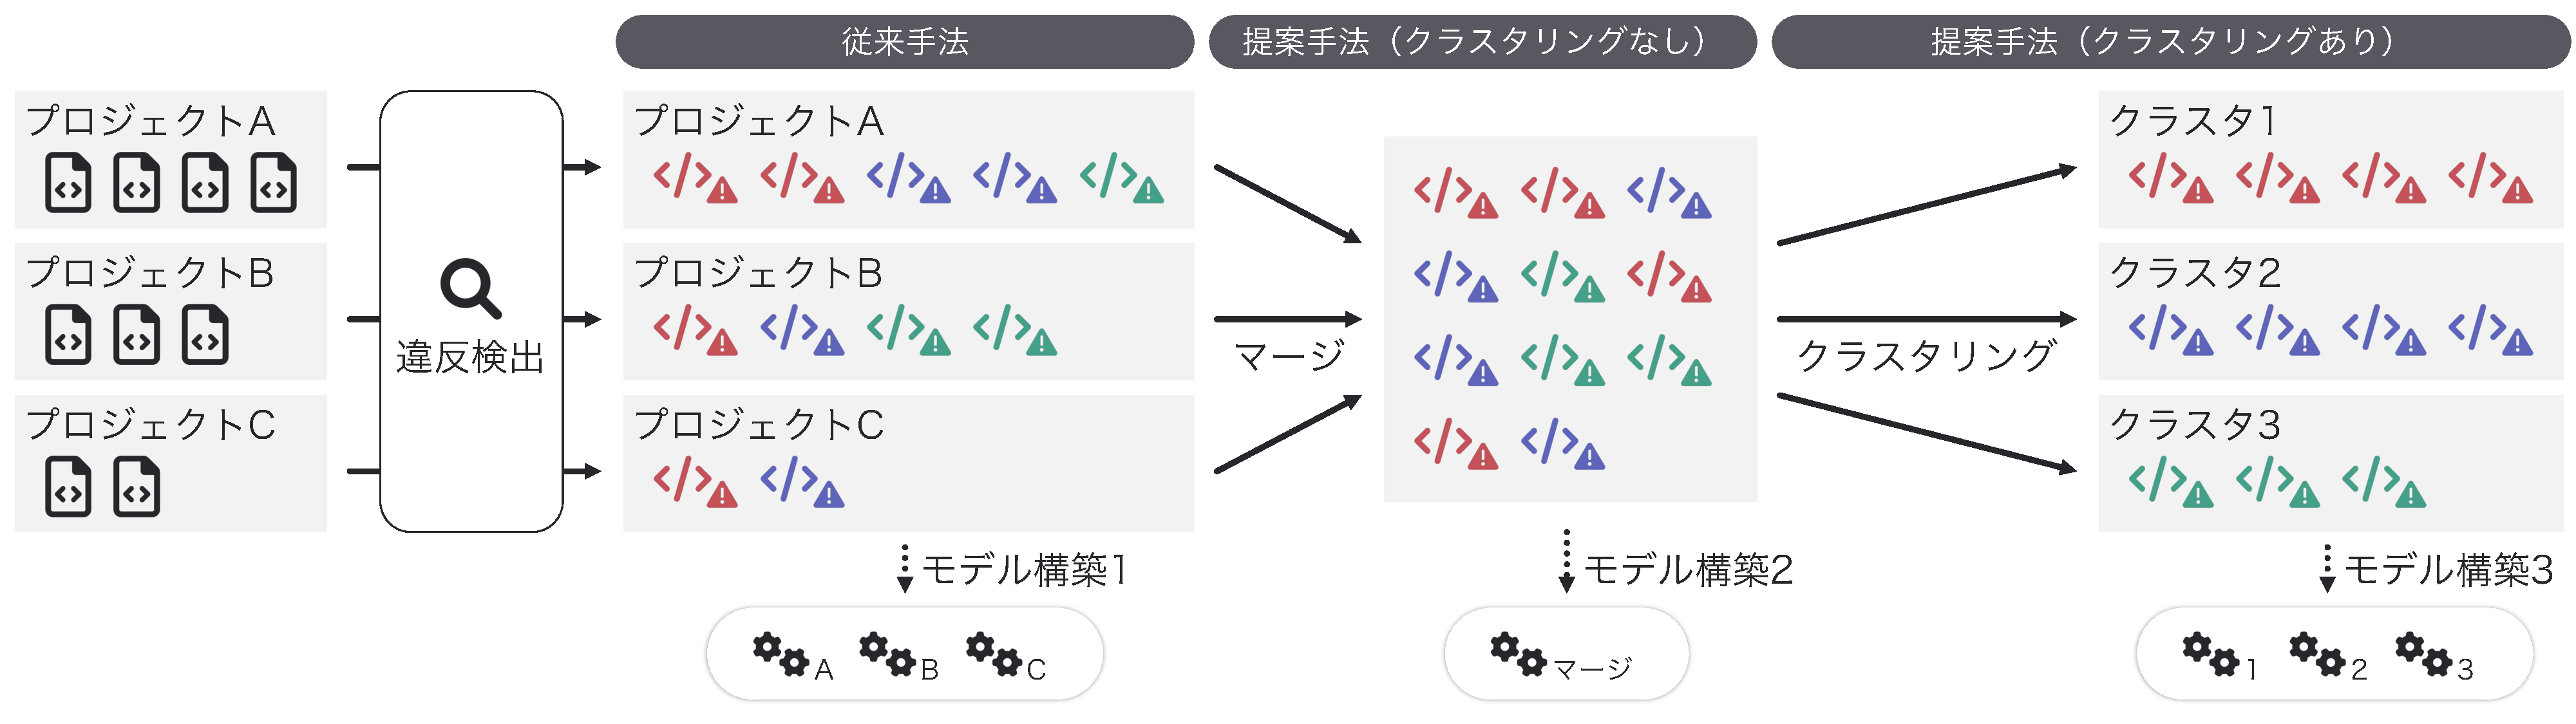
\includegraphics[width=0.8\linewidth]{fig/kameoka_fig1.pdf}
    \caption{提案手法の全体像\todo{(図は更新予定)}}
    \label{fig:Teiannsyuhou}
\end{figure*}
%----------------------

図\ref{fig:Teiannsyuhou}は,本研究で提案する機械学習モデルの構築および評価の概略図を示す.本研究では,予測対象プロジェクトにおける規約違反コードの修正履歴に加え,他のプロジェクトの修正履歴を学習データに含めることにより,修正を要する規約違反コードを予測するモデルを提案する.具体的には3種類のモデル(全学習モデル,選定学習モデル-欠損値補完なし,選定学習モデル-欠損値補完あり)比較手法として,従来研究で提案されている,予測対象プロジェクトにおける修正履歴のみを学習データとして使用する予測モデル(単一学習モデル)も構築し,4つのモデルの予測精度を比較する.

\begin{enumerate}
    \item \textbf{従来手法 - 単一学習モデル}:予測対象のプロジェクトの修正履歴のみを学習データとして用いるモデル\cite{JyuraiPre}.
    \item \textbf{提案手法 - 全学習モデル}:本研究で評価対象とする全てのプロジェクトの修正履歴を学習データとして用いるモデル.
    \item \textbf{提案手法 - 選定学習モデル(欠損値補完なし)}:予測対象プロジェクトの修正履歴に加え,当該プロジェクトが設定する規約,およびその修正率が類似するプロジェクトを選定し,その修正履歴も学習データとして用いるモデル.ただし,プロジェクト間で一方のみが設定する規約の場合,他方の修正率は欠損値であり,本モデルでは\todo{null or 0 or そのIDは類似度算出に使わない?}とする.(選定方法の詳細は\ref{subsec:選定方法}節参照)
    \item \textbf{提案手法 - 選定学習モデル(欠損値補完あり)}:選定学習モデル(欠損値補完なし)と同様に予測対象プロジェクトの修正履歴に加え,選定したプロジェクトの修正履歴も学習データとして用いるモデル.ただし,欠損値は,欠損値を含むプロジェクトにおいて他の規約における平均修正率で補完する.(選定方法の詳細は\ref{subsec:選定方法}節参照)
\end{enumerate}

全学習モデルは,学習データ(特に正例データ)が増加するため精度向上が期待される.その一方で,本研究で評価対象とするプロジェクトには規約違反コードの修正傾向が異なるプロジェクトも含まれるため,精度が低下する可能性もある.

% コーディングスタイルの異なるプロジェクトを含めた学習となるため,それらがノイズとなり,予測精度の低下を招く可能性がある.一方で,複数プロジェクトの修正履歴を活用した予測手法はこれまで提案されておらず,その有効性を明らかにする意義は大きい.

選定学習は,規約違反コードの修正傾向が類似するプロジェクトのみを学習データとして使用するため,正例データを拡張することで,予測精度の向上を期待する.ただし,修正傾向が類似するプロジェクトの選定において,一方のプロジェクトのみが使用する規約は他方のプロジェクトでは欠損値となるため,欠損値補完を用いて類似するプロジェクトを選定する.

% ノイズ低減のために,予測対象プロジェクトと修正傾向が類似したプロジェクトのみを選定する.この際,プロジェクト間の修正傾向の類似性を測定する方法として,複数の類似度指標を用いる.また,欠損値の補完有無による影響も検証対象とする.

% これら3モデルの構築と評価を通じて,コーディング規約違反の修正要否予測における,複数プロジェクトを用いた学習手法の有効性を検証する.



\subsection{説明変数・目的変数の計測方法}

\begin{figure}[t]
    \centering
    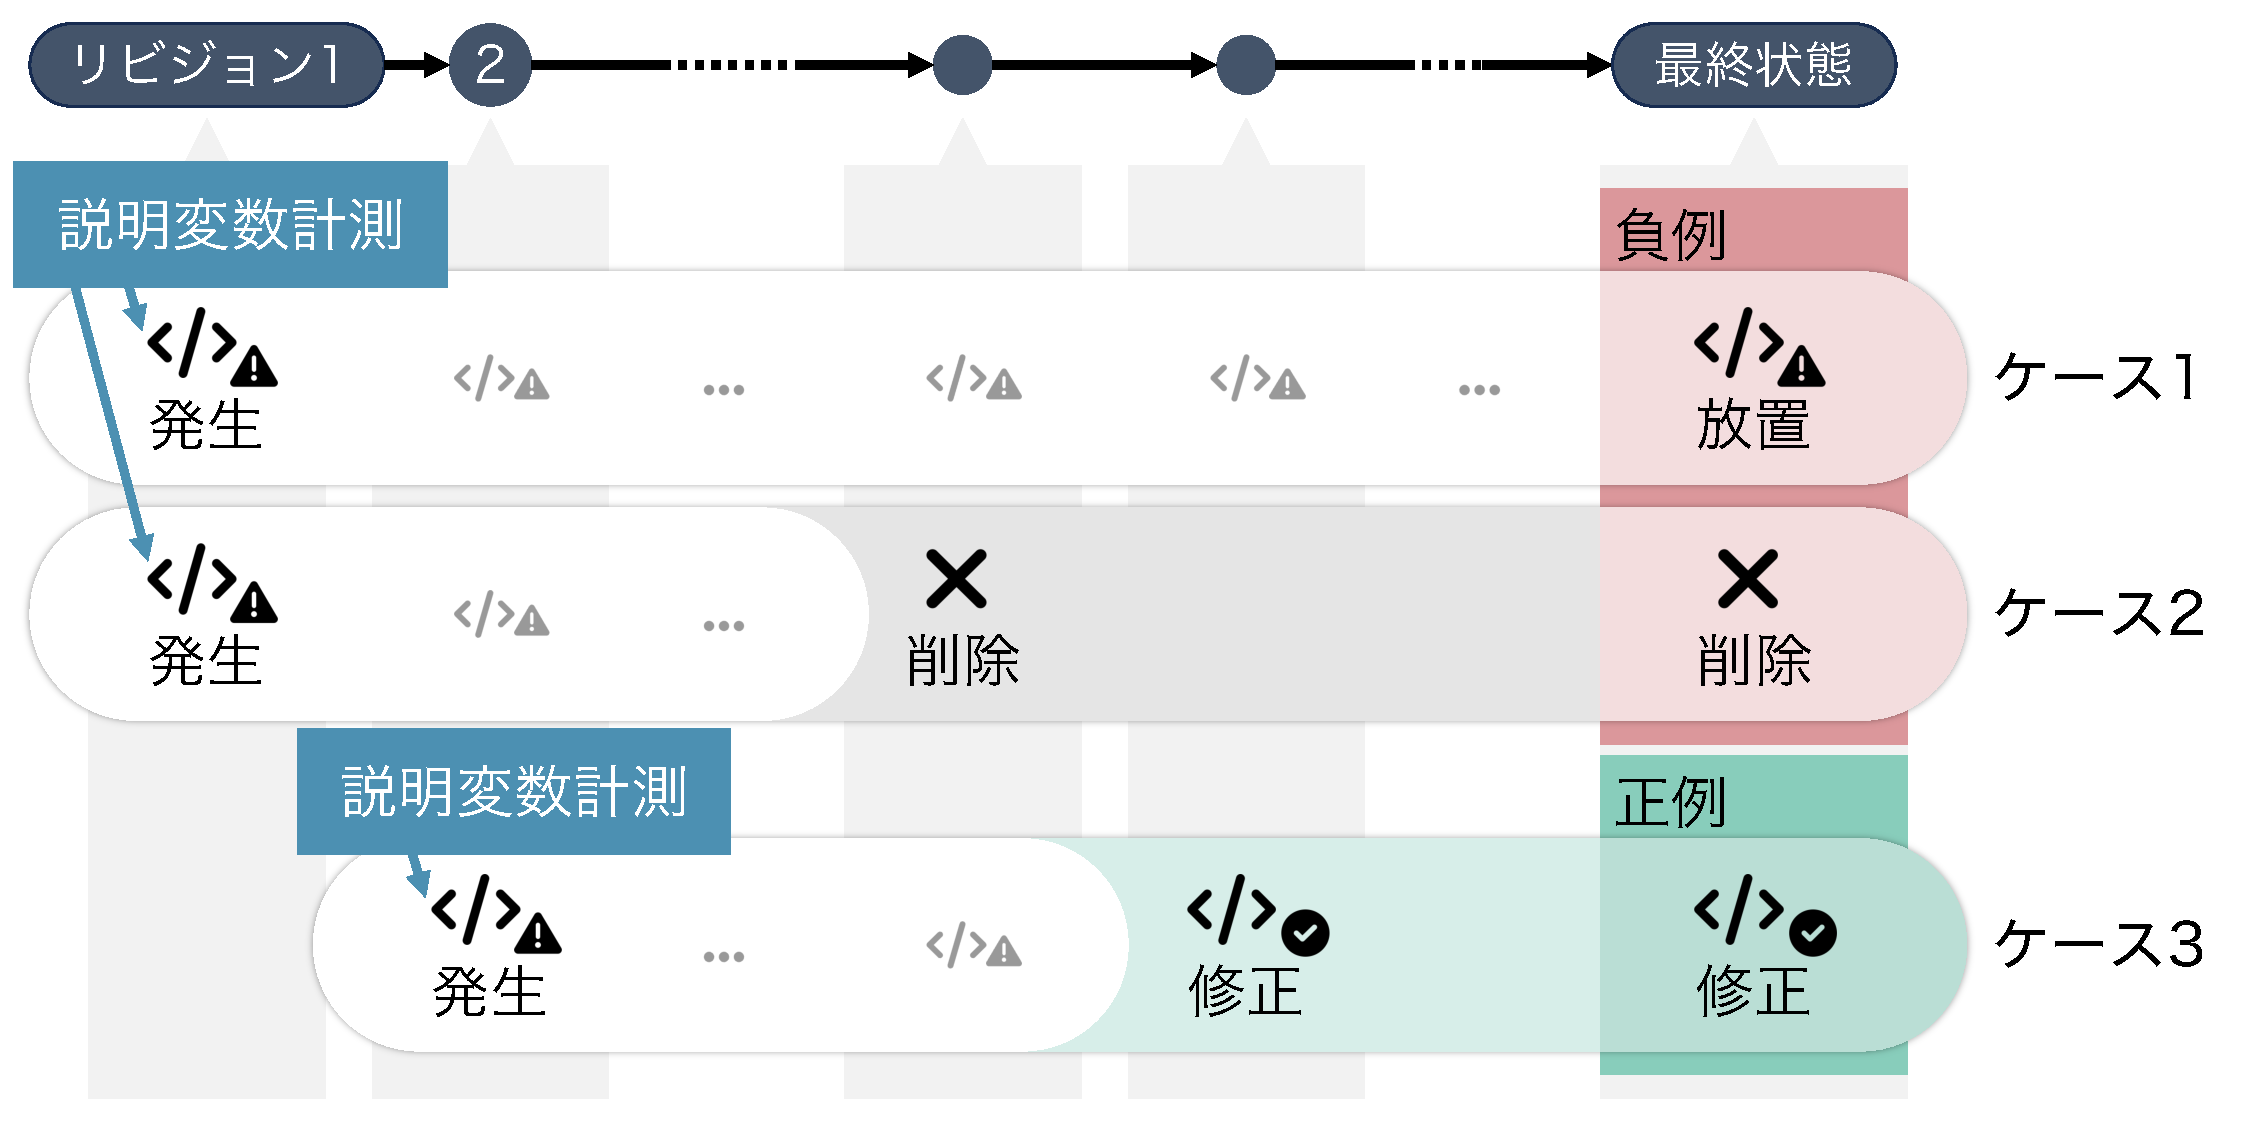
\includegraphics[width=1.0\linewidth]{fig/kameoka_fig2.pdf}
    \caption{説明変数と目的変数の計測位置}
    \label{fig:mokutekihensu}
\end{figure}

図\ref{fig:mokutekihensu}は,本研究で構築するモデルの説明変数および目的変数の計測位置を示す.
説明変数は,規約違反が初めて検出されたリビジョンのソースコード\todo{リポジトリに含まれる他のソースコードからは計測する?しない?}から計測した特徴量43種(行数,コメント行数,循環的複雑度など)を使用する.ソースコードの特徴量は,テクマトリックス社の静的解析ツールUnderstand4.0\footnote{Understand4.0:\url{https://www.techmatrix.co.jp/product/understand/index.html}}を用いて取得する.加えて,\todo{X種の}規約違反IDをOne-hotベクトルとしてを加えた計\todo{X}種の特徴量を説明変数とする.

目的変数は,分析期間内に検出した規約違反コードが,分析期間の最終リビジョンまでに修正される(正例)か否か(負例),言い換えると静的解析ツールにより規約違反として検出されない否かと定義する.
表\ref{tab:pos_neg}は,図\ref{fig:mokutekihensu}に示す3つのケースを例として,目的変数の分類を示す.ケース1およびケース2は負例,ケース3は正例とする.

\begin{table}[t]
    \centering
    \caption{目的変数の正例と負例の分類}
    \label{tab:pos_neg}
    \scalebox{0.85}{
    \begin{tabular}{l|l}
        \hline
        分類 & 説明 \\ \hline
        負例(ケース1) & 規約違反がそのまま残存しているコード断片 \\
        負例(ケース2) & 違反コードが修正されることなく削除された断片 \\
        正例(ケース3) & 規約違反が修正されたコード断片 \\ \hline
    \end{tabular}
    }
\end{table}

% 説明変数は,ソースコードに関する特徴量43種(行数,コメント行数,循環的複雑度など)と,規約違反IDのOne-hotベクトルを加えた計44種である.これらの特徴量は,テクマトリックス社の静的解析ツールUnderstandを用いて取得する.




\subsection{機械学習モデルの構築と評価}

本研究では,従来研究において頻繁に使用されるRandom Forestを予測アルゴリズムとして使用する.従来研究において,規約違反コードの修正要否判定モデルに使用されるデータセットは正例が少ない不均衡データであることが知られている\todo{引用}.この問題に対応するため,各モデルの構築においては,Pythonの機械学習パッケージに実装されているクラス重み付け(\texttt{class\_weights})のオプションを用いる.また,十分な学習\todo{十分な学習ではなく,ランダム性による結果のブレを抑えるため,交差検証で性能を安定化させるためではない?}を確保するために,反復回数は10,000回に設定する.



\subsection{学習プロジェクトの選定方法} \label{subsec:選定方法}

全学習モデル1種および選定学習モデル2種では,予測対象プロジェクトの修正履歴に加え,他のプロジェクトの修正履歴も学習データに含めることにより正例データを拡張する.全学習モデルではデータセット内の全プロジェクトを対象とし,選定学習モデルでは,予測対象プロジェクトが設定する規約,およびその修正率が類似するプロジェクトの修正履歴のみを学習データに含める.\todo{プロジェクト間の類似度にIDごとに取り組んでいる研究はある?ID別に計測することの動機をここで書きたい.}本研究では,各プロジェクトで収集するコミット履歴のうち,古い履歴8割を学習データとし,新しい2割を検証データとする.プロジェクト選定は,学習データにおいて予測対象プロジェクトが設定する規約,およびその修正率を計測し,他のプロジェクトとの類似度を算出する.プロジェクトの選定方法は,予測対象プロジェクトと類似するコーディング規約違反を設定していること,またその修正率が類似していることとする.各規約違反における修正率の算出式は式(\ref{eq:fixrate})に示す.

\begin{equation}
\label{eq:fixrate}
\text{修正率} = \frac{\text{違反の修正された数}}{\text{違反を検出した数}}
\end{equation}

プロジェクト間の類似度は,各プロジェクトが設定する規約の類似度,および規約の修正率の類似度をそれぞれ算出する.各プロジェクトが設定する規約の類似度は,本研究で対象とするPylintで設定可能な\todo{N}種類の規約を対象とし,プロジェクトの規約設定有無(バイナリーデータ)の類似度を判定するためジャッカード係数を用いる.修正率の類似度はは,各プロジェクトが設定する個々の規約の修正率(スカラーデータ)の類似度を判定するためユークリッド距離を用いる.プロジェクト間でそれぞれの指標が類似するか否かは,実証データに基づき閾値を決定する.

% 修正率を基に,ジャッカード係数とユークリッド距離の2種類の類似度指標を算出し,それぞれに閾値を設定することで,類似度が高いと判断されたプロジェクトのみを学習対象として選定する.
なお,規約の修正率は,一方のプロジェクトのみが規約を設定している場合,他方のプロジェクトでは欠損値となるため,次の2通りの方法で欠損値補完し,類似度を計測する.

%ユークリッド距離の計算においては,ある規約違反が一度も発生していない場合,修正率が欠損値となる.この場合に備え,以下の2通りの処理を実施する.
\begin{itemize}
    \item 欠損値を計算から除外してユークリッド距離を測定する方法(選定学習モデル(欠損値補完なし))
    \item 欠損値を当該プロジェクトの平均修正率で補完し,ユークリッド距離を測定する方法(選定学習モデル(欠損値補完あり))
\end{itemize}

欠損値の補完方法には様々な手法が提案されているが,規約違反コードの修正要否を予測するモデルにおいて,複数のプロジェクトの修正履歴を統合する従来研究が確認できないため,本研究の結果に基づき他の欠損値補完手法を検討する.

%XXの類似度は,ジャッカード係数を0.1から0.5まで0.1刻み,ユークリッド距離は1.5から5.0まで0.5刻みとし,その組み合わせを網羅的に検証する.各指標における最小・最大の閾値は,全プロジェクトが含まれる境界または全く含まれない境界として設定している.\todo{境界の意味が伝わらない}


%%%%%%%%%%%%%%%%%%%%%%%%%%%
\section{ケーススタディ}\label{chap:result}
%%%%%%%%%%%%%%%%%%%%%%%%%%%

\subsection{データセット}

\begin{table}[t]
    \centering
    \caption{データセット統計量\todo{おそらく削除.\ref{table:result1}に含めるため.}}
    \label{tab:dataset_statistics}
    \begin{tabular}{ccc}
        \toprule
        総データ平均値 & 正例数平均値 & 負例数平均値 \\
        \midrule
        4,465 & 1,147 & 3,318 \\
        \bottomrule
    \end{tabular}
\end{table}

ケーススタディとして,ライブラリ検索サービスであるLibraries.io\footnote{\url{https://libraries.io/}}に登録されているプロジェクトから,主要言語がPython,静的解析ツールとしてPylintを利用,GitHub上でソースコードと規約違反修正履歴を公開しているリポジトリを対象とする.特に,SourceRank上位1,500プロジェクトの中から,Pylintの設定ファイル(\texttt{pylintrc}または\texttt{.pylintrc})を有し,学習・評価データの双方に正例・負例が含まれていた20プロジェクトを選定した.表\ref{table:result1}の左から1列目にプロジェクト一覧を示す.各プロジェクトにおいて2018年12月から1,000日間のコミット履歴を対象とする.
% 表\ref{tab:dataset_statistics}に示すとおり,本データセットでは負例の数が正例の約3倍となっており,クラス間の不均衡が顕著である.


% Pythonを実験対象言語とした理由は,近年,機械学習やデータ分析における需要の高まりを背景に,Pythonの重要性が増しているためである.また,JavaやC言語に比べて,本分野における予測研究が少ないことも理由の一つである.

% \subsection{実験結果}



\subsection{予測精度の評価結果}

%---------------------
\begin{table*}[t]
  \centering
  \caption{手法別の予測精度}
  \label{table:result1}
  \resizebox{\textwidth}{!}{%
  \begin{tabular}{lcccccccccccc}
    \toprule
    \multirow{2}{*}{プロジェクト名} 
    & \multicolumn{3}{c}{単一学習} 
    & \multicolumn{3}{c}{全学習} 
    & \multicolumn{3}{c}{選定学習} 
    & \multicolumn{3}{c}{\shortstack{選定学習\\(欠損値補完あり)}} \\
    \cmidrule(lr){2-4} \cmidrule(lr){5-7} \cmidrule(lr){8-10} \cmidrule(lr){11-13}
    & 適合率 & 再現率 & F1値 & 適合率 & 再現率 & F1値 & 適合率 & 再現率 & F1値 & 適合率 & 再現率 & F1値 \\
    \midrule
        sockeye & 0.75 & \textbf{\underline{0.83}} & \textbf{\underline{0.79}} & 0.75 & 0.81 & 0.78 & \textbf{\underline{0.77}} & 0.82 & 0.79 & 0.75 & \textbf{\underline{0.83}} & \textbf{\underline{0.79}} \\
        coretools & 0.14 & 0.24 & 0.18 & 0.07 & 0.39 & 0.12 & 0.05 & 0.07 & 0.06 & 0.14 & 0.24 & 0.18 \\
        \underline{howdoi} & 0.78 & 0.99 & 0.87 & 0.07 & 0.97 & 0.13 & 0.72 & 0.99 & 0.84 & 0.72 & 0.99 & 0.84 \\
        schema\_salad & 0.66 & 0.58 & 0.62 & 0.59 & 0.22 & 0.32 & 0.66 & 0.36 & 0.47 & 0.66 & 0.58 & 0.62 \\
        serverless-application-model & 0.72 & 0.27 & 0.39 & 0.74 & 0.20 & 0.32 & 0.77 & 0.32 & 0.45 & 0.72 & 0.27 & 0.39 \\
        SoCo & 0.67 & 0.64 & 0.66 & 0.74 & 0.54 & 0.62 & 0.70 & 0.61 & 0.65 & 0.67 & 0.64 & 0.66 \\
        behave & 0.33 & 0.37 & 0.35 & 0.26 & 0.35 & 0.30 & 0.33 & 0.24 & 0.28 & 0.33 & 0.37 & 0.35 \\
        OWSLib & 0.61 & 0.77 & 0.68 & 0.63 & 0.77 & 0.69 & 0.62 & 0.77 & 0.68 & 0.61 & 0.77 & 0.68 \\
        pynput & 0.34 & 0.87 & 0.49 & 0.47 & 0.54 & 0.50 & 0.31 & 0.75 & 0.44 & 0.34 & 0.87 & 0.49 \\
        schematics & 0.44 & 0.75 & 0.55 & 0.45 & 0.77 & 0.57 & 0.45 & 0.74 & 0.56 & 0.44 & 0.75 & 0.55 \\
        \underline{hickle} & 0.14 & 0.14 & 0.14 & 0.24 & 0.53 & 0.33 & 0.24 & 0.55 & 0.33 & 0.13 & 0.17 & 0.15 \\
        \underline{python-sdk} & 0.43 & 0.45 & 0.44 & 0.31 & 0.63 & 0.41 & 0.44 & 0.71 & 0.54 & 0.43 & 0.63 & 0.51 \\
        rtv & 0.73 & 0.51 & 0.60 & 0.62 & 0.33 & 0.43 & 0.71 & 0.51 & 0.60 & 0.73 & 0.51 & 0.60 \\
        datadogpy & 0.02 & 0.05 & 0.03 & 0.13 & 0.46 & 0.20 & 0.12 & 0.33 & 0.17 & 0.02 & 0.05 & 0.03 \\
        pychromecast & 0.93 & 0.89 & 0.91 & 0.87 & 0.75 & 0.81 & 0.90 & 0.88 & 0.89 & 0.93 & 0.89 & 0.91 \\
        \underline{pyscard} & 0.08 & 0.17 & 0.11 & 0.07 & 0.50 & 0.12 & 0.06 & 0.33 & 0.10 & 0.12 & 0.33 & 0.18 \\
        imgaug & 0.10 & 0.05 & 0.07 & 0.50 & 0.02 & 0.03 & 0.10 & 0.05 & 0.07 & 0.10 & 0.05 & 0.07 \\
        \underline{GPflow} & 0.64 & 0.89 & 0.74 & 0.61 & 0.18 & 0.28 & 0.64 & 0.82 & 0.72 & 0.65 & 0.90 & 0.75 \\
        \underline{transitions} & 0.83 & 0.96 & 0.89 & 0.82 & 0.98 & 0.89 & 0.81 & 0.98 & 0.89 & 0.84 & 0.96 & 0.89 \\
        pyphi & 0.67 & 0.78 & 0.72 & 0.69 & 0.92 & 0.79 & 0.67 & 0.78 & 0.72 & 0.67 & 0.78 & 0.72 \\
    \bottomrule
  \end{tabular}
  }
\end{table*}
%---------------------

%---------------------
\begin{figure}[t]
	\centering
        % 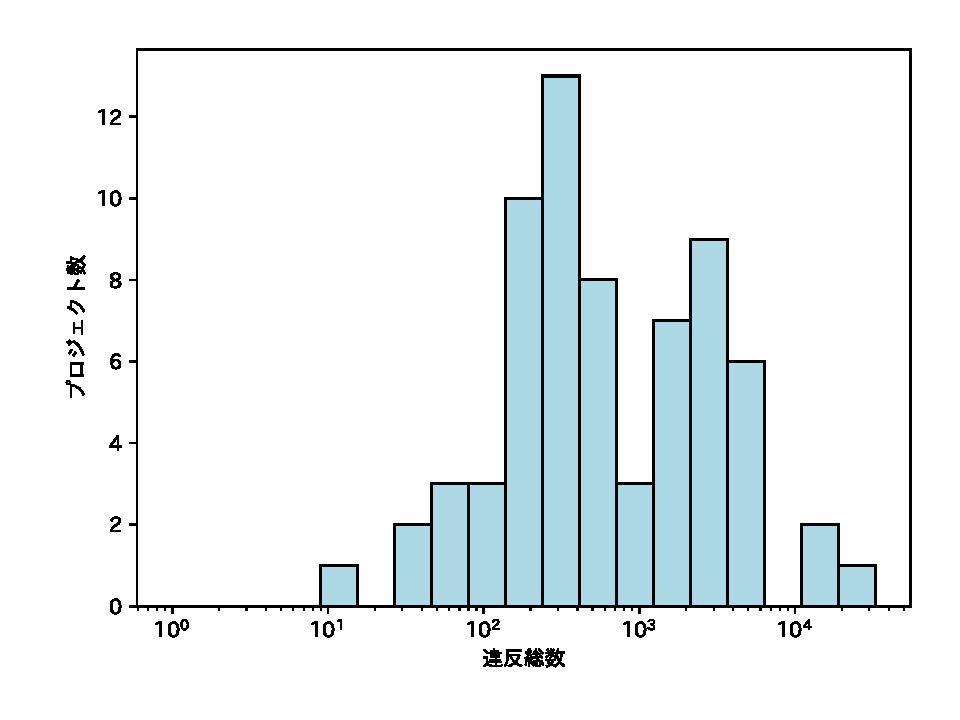
\includegraphics[width=0.25\textwidth, bb=0 0 4 3]{fig/dataset_hist.pdf}
	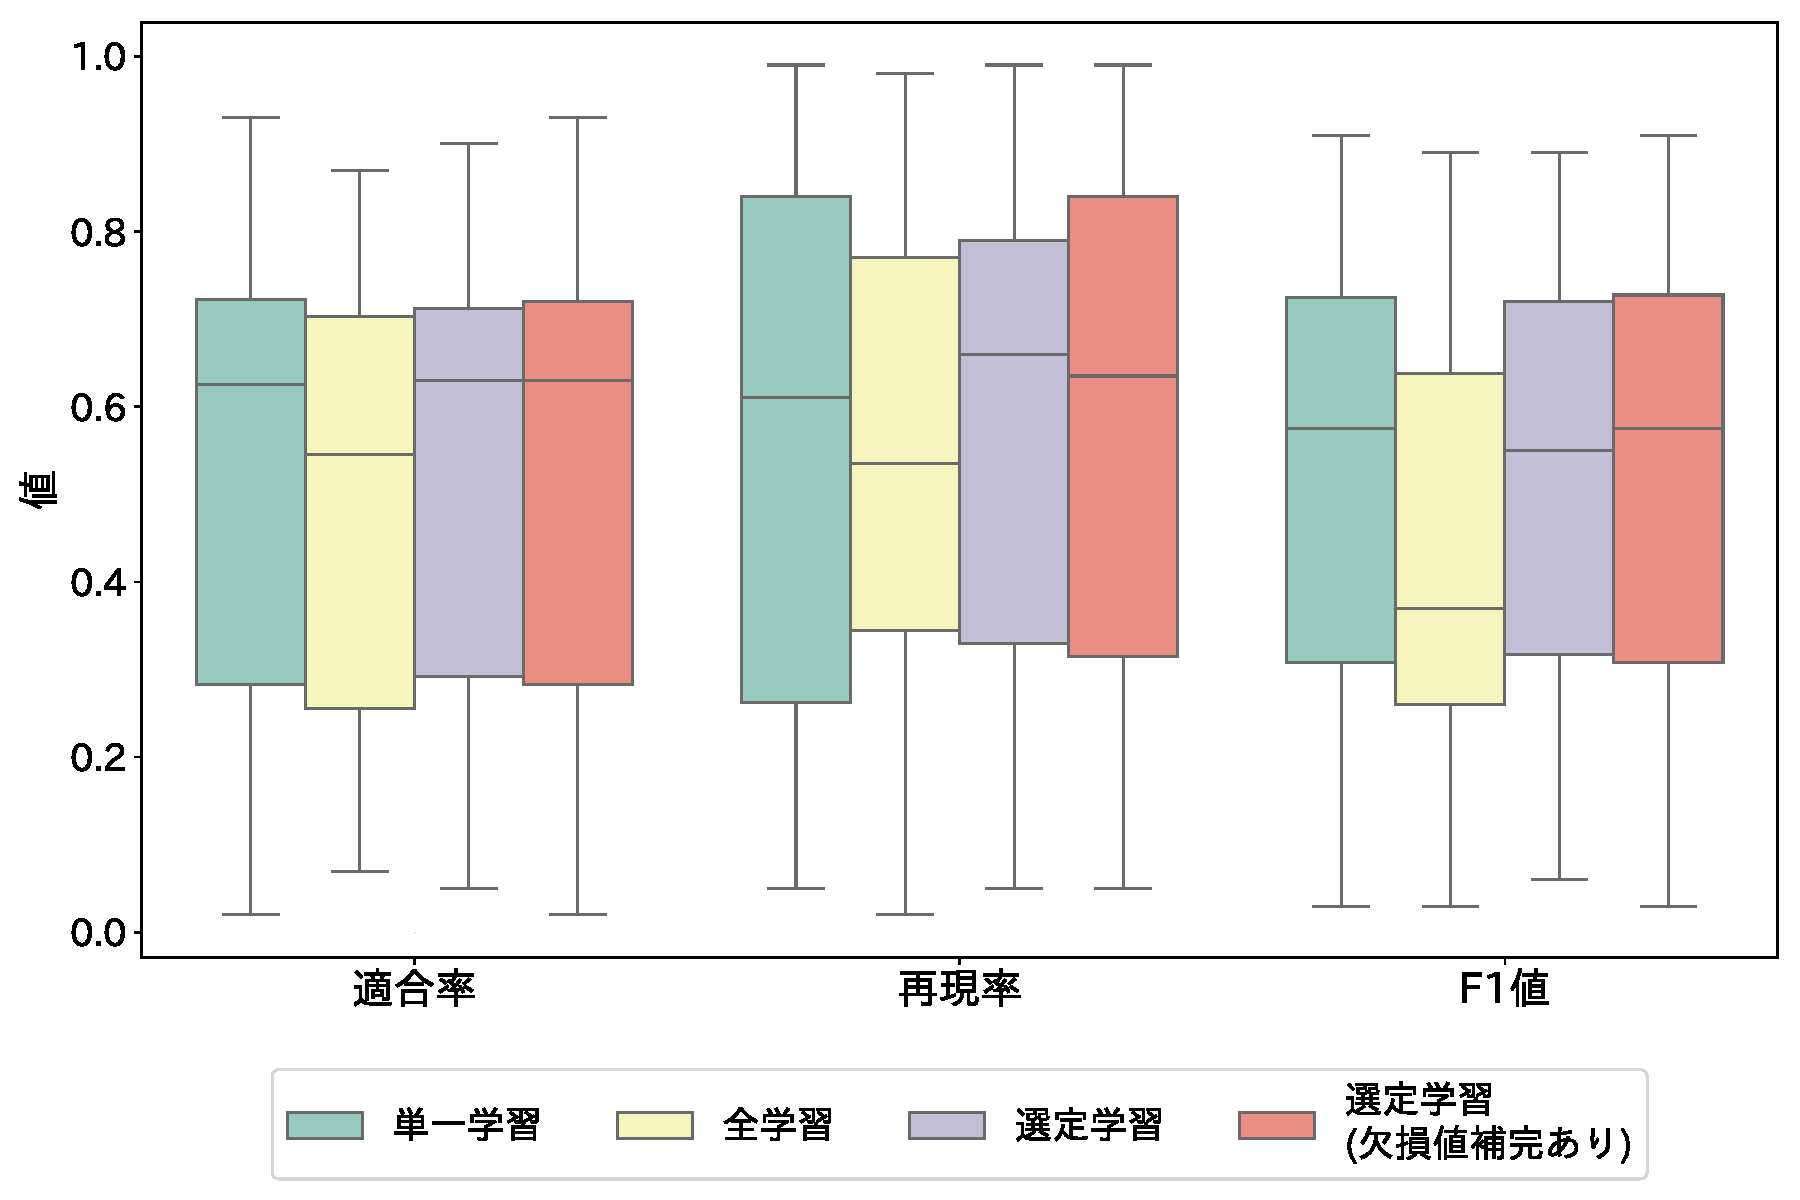
\includegraphics[width=1\linewidth]{fig/boxplot_unfiltered.pdf}
	\caption{4手法による予測結果の箱ひげ図}
	\label{fig:boxplot}


	\centering
        % 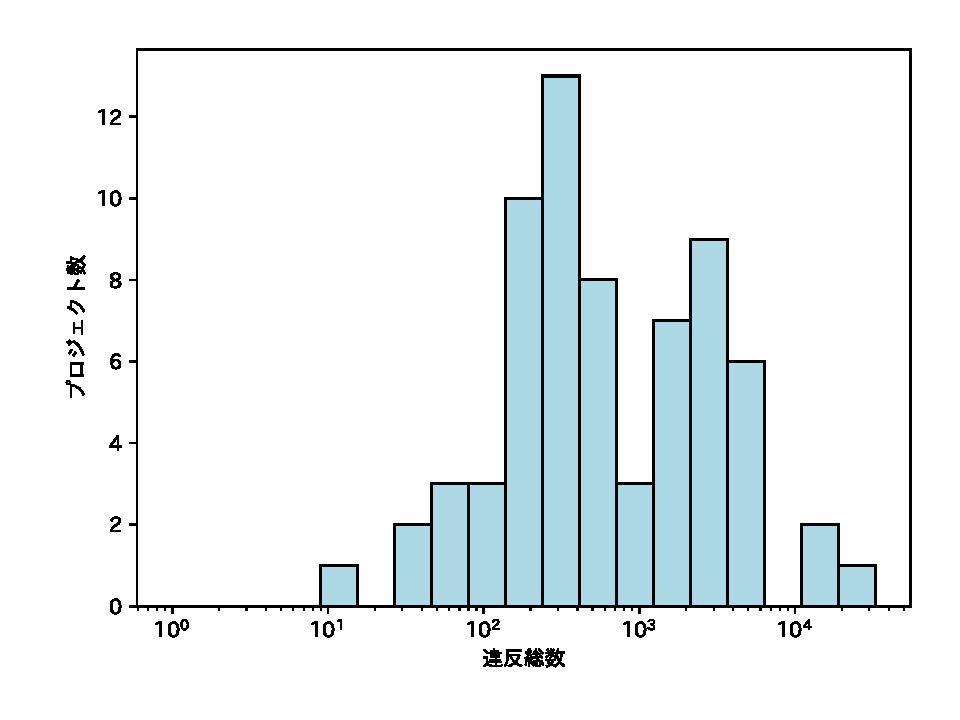
\includegraphics[width=0.25\textwidth, bb=0 0 4 3]{fig/dataset_hist.pdf}
	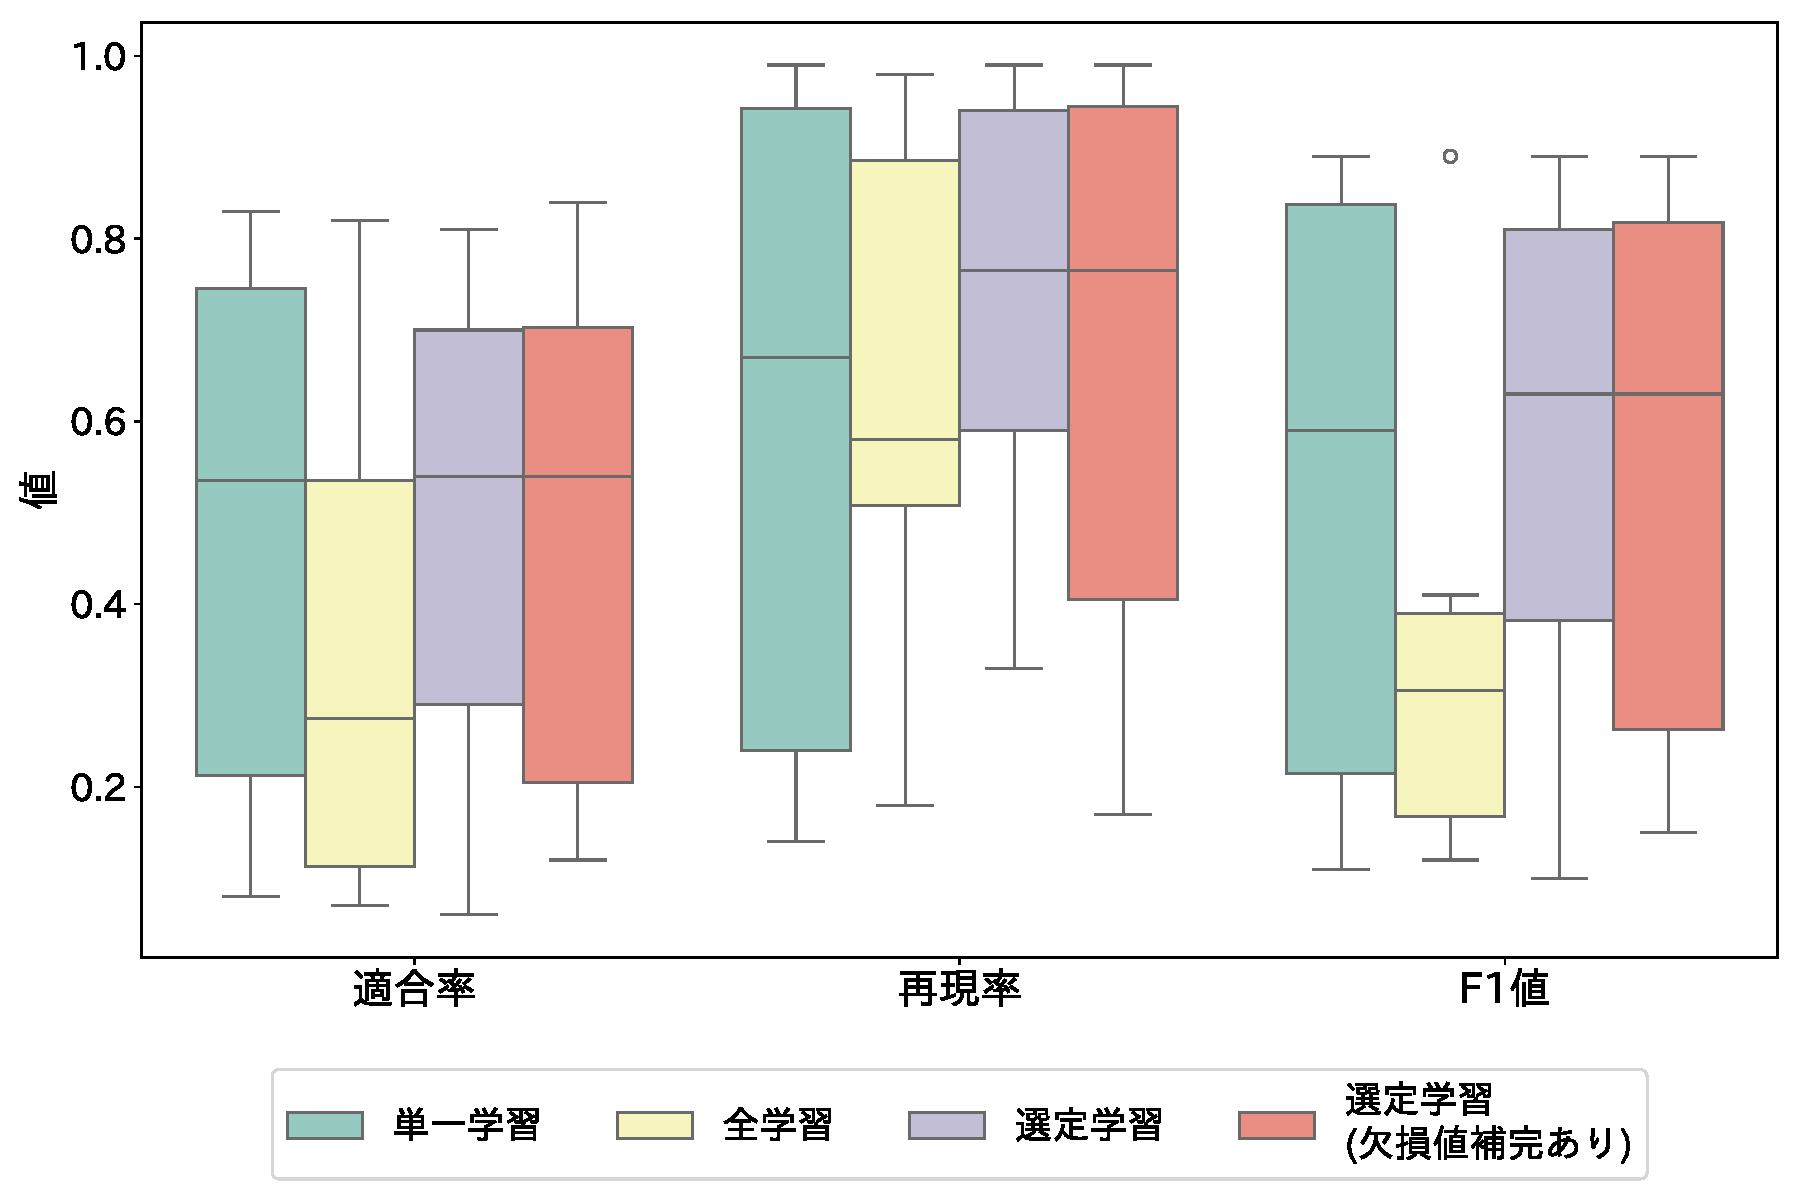
\includegraphics[width=1\linewidth]{fig/boxplot_filtered.pdf}
	\caption{選定学習手法(欠損値補完あり)で複数プロジェクトのデータを学習したプロジェクトに絞った予測結果の箱ひげ図}
	\label{fig:boxplot_filtered}
\end{figure}
%---------------------

表\ref{table:result1}は,従来研究の予測モデル1種類,および本研究で提案する予測モデル3種類の予測精度を示す.左の列から,予測対象プロジェクト名,\todo{正例数(?),負例数(?)}を示し,さらに手法別の適合率,再現率,F1値を示す.図\ref{fig:boxplot}は,表\ref{table:result1}に示した結果を手法別に箱ひげ図で示す.

選定学習モデルは,プロジェクトが設定する規約の類似度,およびその修正率の類似度を算出し,プロジェクト間で類似すると判定する閾値を変更し,予測精度が最も高かった値を表\ref{table:result1}に示す.具体的には,プロジェクトが設定する規約の類似度はジャッカード係数を0.1から0.5まで0.1刻み,修正率の類似度はユークリッド距離は1.5から5.0まで0.5刻みに変更し,その組み合わせを網羅的に検証した.その結果,選定学習モデル(欠損値補完なし)はジャッカード係数0.3以下,ユークリッド距離3.0以下,選定学習(欠損値補完あり)はジャッカード係数:0.3以下,ユークリッド距離:3.5以下で最も高い予測精度であった.\todo{これはグラフ出すとすごい量になる?}\todo{このスコアについては考察したほうが良さそう}欠損値補完することにより,1つ以上のプロジェクトの修正履歴を統合したのは,表\ref{table:result1}のプロジェクト名に下線のある6プロジェクトのみであったため,表\ref{table:result1}に当該6プロジェクト以外のプロジェクトは選定学習モデル(欠損値補完あり)の予測精度は掲載していない.\todo{図\ref{fig:boxplot}から選定学習モデル(欠損値補完あり)を消してはどうだろう?}\todo{6プロジェクトは何と(またはどんなプロジェクトと)統合したのだろう?考察で言及?}

図\ref{fig:boxplot}から,F1値は提案手法(全学習モデル)が従来手法(単一学習モデル)と提案手法(選定学習モデル2種類)に比べて低く,表\ref{table:result1}から分析対象20プロジェクト中15プロジェクトにおいて全学習モデルのF1値が他のモデルより低い\todo{検定した?}.この結果は著者らも予想していた結果であり,評価対象とするプロジェクトには規約違反コードの修正傾向が異なるプロジェクトが多数含まれていたことが示唆される.todo{修正傾向についてはX章で考察する.}

再現率は提案手法(選定学習モデル2種類)が,提案手法(全学習モデル)と従来手法(単一学習モデル)に比べて向上する\todo{検定した?}.ただし,選定学習モデル2種類は欠損値補完の有無によって予測精度に有意な差はみられなかった.\todo{次の文章は図3の修正次第で削除する}その理由は,選定学習モデルで対象とする20プロジェクトのうち,欠損値補完を経て他のプロジェクトの修正履歴を学習データに含むプロジェクトは6プロジェクトのみであり,その他の14プロジェクトは同じ予測結果であるためである.

図\ref{fig:boxplot_filtered}は,他のプロジェクトを使って学習データを拡張した6プロジェクトに関する4種類のモデルの予測結果を箱ひげ図で示す.図\ref{fig:boxplot}とおよそ同じ結果であるが,全学習モデルによる精度低下が顕著となり,選定学習モデルの再現率とF1値が単一学習モデルよりも高く,統計的に有意な差があることがわかった.\todo{要検定}

% 選定学習モデル(欠損値補完あり)において,複数プロジェクトの学習データを統合して学習していた6プロジェクトに絞り,予測結果を箱ひげ図にしたものを図\ref{fig:boxplot_filtered}に示す.
% 図\ref{fig:boxplot_filtered}から,欠損値補完の有無によらず,選定学習では,単一学習と比較して,適合率を維持した状態で,再現率が改善されている.また,再現率が向上したことによるF1値の向上も見られる.
% また,再現率においては,全学習においても,中央値では単一学習より低下しているが,最小値や第一四分位数が改善している.



% 図\ref{fig:boxplot}から,選定学習の予測結果に注目すると,全学習の結果と比較して予測精度の改善が見られる.再現率の中央値に関しては,従来手法である単一学習からわずかに改善が見られる.
% しかし,適合率とF1値に関しての予測精度の変化は見られない.

% 最後に選定学習(欠損値補完あり)の結果について述べる.図\ref{fig:boxplot}から,選定学習(欠損値補完あり)の結果は,欠損値補完を行わない選定学習手法から大きな変化がないことがわかる.この結果の要因として,選定学習(欠損値補完あり)において,複数プロジェクトの学習データを統合して学習していたプロジェクトが,6プロジェクトのみであることが要因の一つとして考えられる.
% 複数プロジェクトのデータを学習に利用していた,予測対象プロジェクトは表\ref{table:result1}のプロジェクト名に下線を引いている6プロジェクトである.
% % つまり,下線が引かれていない14プロジェクトでは,類似しているプロジェクトが無いという結果となり,予測対象プロジェクトの過去のデータのみを利用した単一学習と同じ結果となり,変化があまり見られない結果となっている.
% そこで,選定学習(欠損値補完あり)において,複数プロジェクトの学習データを統合して学習していた6プロジェクトに絞り,予測結果を箱ひげ図にしたものを図\ref{fig:boxplot_filtered}に示す.
% 図\ref{fig:boxplot_filtered}から,欠損値補完の有無によらず,選定学習では,単一学習と比較して,適合率を維持した状態で,再現率が改善されている.また,再現率が向上したことによるF1値の向上も見られる.
% また,再現率においては,全学習においても,中央値では単一学習より低下しているが,最小値や第一四分位数が改善している.

\begin{screen}
他のプロジェクトの修正履歴を用いて学習データを拡張することで再現率が向上する一方,全学習のようにプロジェクトの修正傾向を無視した単に学習データの統合を行うだけでは,適合率,F1値が低下するため,統合するプロジェクトを選定して,学習データを拡張する必要がある.\todo{表の修正次第で,正例数を増やした効果と言い換えたい.次の節の説明のためにも.}
\end{screen}


\subsection{提案手法により予測精度が向上するプロジェクトの調査}

% sockeye: ['hickle', 'pyscard', 'transitions']
% coretools: ['hickle', 'pyscard']
% howdoi: ['pyscard']
% schema_salad: ['hickle', 'pyscard']
% serverless-application-model: ['OWSLib', 'pynput', 'schematics', 'hickle', 'python-sdk', 'datadogpy', 'pyscard', 'transitions']
% SoCo: ['pynput', 'schematics', 'hickle', 'python-sdk', 'GPflow', 'transitions', 'pyphi']
% behave: ['pynput', 'hickle']
% OWSLib: ['serverless-application-model', 'hickle', 'datadogpy', 'pyscard']
% pynput: ['serverless-application-model', 'SoCo', 'behave', 'schematics', 'hickle', 'python-sdk', 'datadogpy', 'GPflow', 'transitions', 'pyphi']
% schematics: ['serverless-application-model', 'SoCo', 'pynput', 'hickle', 'python-sdk', 'datadogpy', 'GPflow', 'pyphi']
% hickle: ['coretools', 'schema_salad', 'serverless-application-model', 'SoCo', 'behave', 'OWSLib', 'pynput', 'schematics', 'rtv', 'datadogpy', 'pyscard', 'GPflow', 'transitions', 'pyphi']
% python-sdk: ['serverless-application-model', 'SoCo', 'pynput', 'schematics', 'rtv', 'datadogpy', 'pychromecast', 'GPflow', 'transitions', 'pyphi']
% rtv: ['hickle', 'python-sdk']
% datadogpy: ['serverless-application-model', 'OWSLib', 'pynput', 'schematics', 'hickle', 'python-sdk', 'pyscard']
% pychromecast: ['python-sdk', 'GPflow']
% pyscard: ['coretools', 'howdoi', 'schema_salad', 'serverless-application-model', 'OWSLib', 'hickle', 'datadogpy']
% GPflow: ['SoCo', 'pynput', 'schematics', 'hickle', 'python-sdk', 'pychromecast', 'transitions']
% transitions: ['serverless-application-model', 'SoCo', 'pynput', 'hickle', 'python-sdk', 'GPflow', 'pyphi']

% === coretools (RandomForest) の重要度上位10カラム ===
%  1. AvgLineBlank                   0.0452
%  2. CountLineBlank                 0.0352
%  3. CountLine                      0.0331
%  4. CountLineComment               0.0326
%  5. CountLineCode                  0.0300
%  6. CountStmt                      0.0278
%  7. CountLineCodeExe               0.0269
%  8. RatioCommentToCode             0.0260
%  9. E0401                          0.0247
% 10. CountStmtExe                   0.0237

% === behave (RandomForest) の重要度上位10カラム ===
%  1. CountLineCode                  0.0528
%  2. CountStmt                      0.0525
%  3. CountLineCodeExe               0.0480
%  4. CountStmtDecl                  0.0460
%  5. AvgLine                        0.0451
%  6. CountLineCodeDecl              0.0443
%  7. W1406                          0.0408
%  8. CountLine                      0.0408
%  9. CountStmtExe                   0.0321
% 10. C0209                          0.0287

% === hickle (RandomForest) の重要度上位10カラム ===
%  1. W0612                          0.0786
%  2. CountLine                      0.0781
%  3. CountLineBlank                 0.0739
%  4. C0209                          0.0547
%  5. C0116                          0.0536
%  6. CountDeclMethodAll             0.0478
%  7. C0305                          0.0298
%  8. E0401                          0.0279
%  9. E0602                          0.0279
% 10. CountStmtExe                   0.0250

% === python-sdk (RandomForest) の重要度上位10カラム ===
%  1. C0209                          0.1187
%  2. R0205                          0.1034
%  3. CountLineCode                  0.0353
%  4. RatioCommentToCode             0.0337
%  5. CountLineCodeExe               0.0335
%  6. CountLine                      0.0321
%  7. CountStmt                      0.0293
%  8. CountLineComment               0.0286
%  9. CountLineCodeDecl              0.0278
% 10. CountStmtExe                   0.0261

% === pyscard (RandomForest) の重要度上位10カラム ===
%  1. E0001                          0.1129
%  2. E0602                          0.0486
%  3. C0121                          0.0449
%  4. AvgLineCode                    0.0431
%  5. C0103                          0.0415
%  6. CountLineCodeDecl              0.0260
%  7. AvgLine                        0.0237
%  8. RatioCommentToCode             0.0232
%  9. CountLineComment               0.0223
% 10. CountLine                      0.0222

% === datadogpy (RandomForest) の重要度上位10カラム ===
%  1. CountLineCodeExe               0.0453
%  2. CountLineCode                  0.0420
%  3. CountStmtExe                   0.0398
%  4. C0301                          0.0396
%  5. RatioCommentToCode             0.0362
%  6. CountLine                      0.0339
%  7. CountStmt                      0.0339
%  8. CountLineBlank                 0.0291
%  9. CountLineComment               0.0258
% 10. C0209                          0.0255

% === howdoi (RandomForest) の重要度上位10カラム ===
%  1. CountLineCodeExe               0.1246
%  2. CountStmtExe                   0.1021
%  3. CountLine                      0.0924
%  4. CountLineCode                  0.0891
%  5. CyclomaticModified             0.0676
%  6. RatioCommentToCode             0.0568
%  7. Essential                      0.0521
%  8. CountClassBase                 0.0484
%  9. Cyclomatic                     0.0447
% 10. CyclomaticStrict               0.0407

% === rtv (RandomForest) の重要度上位10カラム ===
%  1. C0209                          0.0569
%  2. E0401                          0.0400
%  3. CountLineCodeExe               0.0317
%  4. R0914                          0.0301
%  5. R0915                          0.0290
%  6. CountStmt                      0.0276
%  7. CountLine                      0.0271
%  8. CountLineCode                  0.0266
%  9. CountStmtExe                   0.0266
% 10. R1705                          0.0253



% === GPflow (RandomForest) の重要度上位10カラム ===
%  1. C0301                          0.0539
%  2. CountLineCode                  0.0511
%  3. CountLine                      0.0449
%  4. E0401                          0.0436
%  5. C0305                          0.0393
%  6. E0602                          0.0376
%  7. CountStmt                      0.0374
%  8. W0611                          0.0365
%  9. CountLineBlank                 0.0357
% 10. RatioCommentToCode             0.0331

% === transitions (RandomForest) の重要度上位10カラム ===
%  1. C0209                          0.0982
%  2. CountLine                      0.0353
%  3. CountLineCodeExe               0.0347
%  4. CountStmt                      0.0326
%  5. CountLineCode                  0.0319
%  6. SumCyclomaticModified          0.0313
%  7. C0103                          0.0308
%  8. C0411                          0.0300
%  9. CountLineCodeDecl              0.0299
% 10. CountStmtExe                   0.0295


%----------------------
\begin{figure}[t]
	\centering
        % 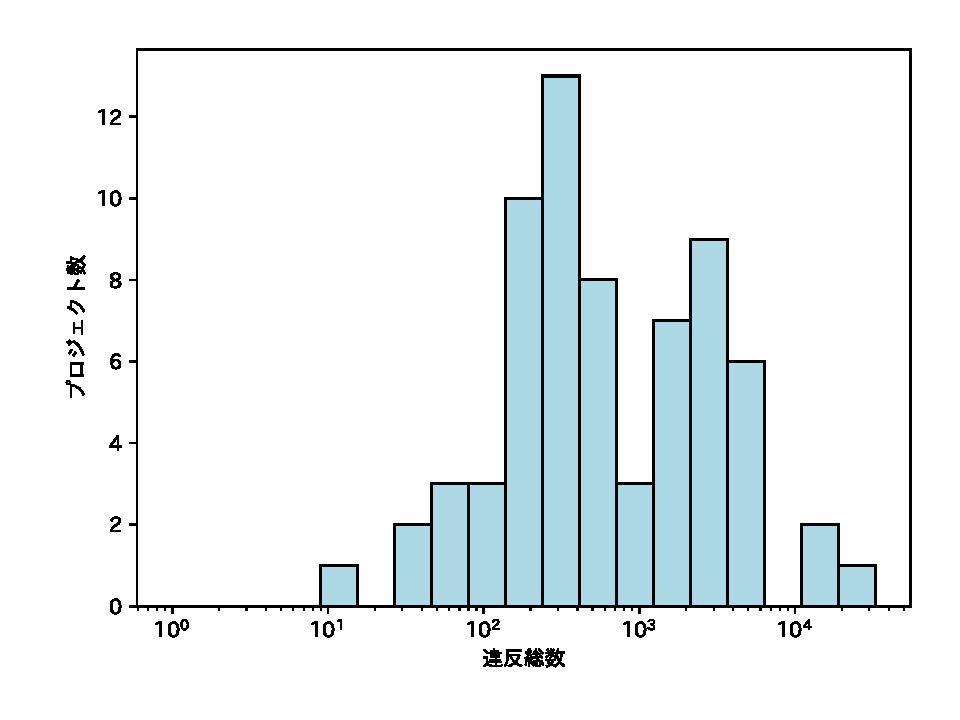
\includegraphics[width=0.25\textwidth, bb=0 0 4 3]{fig/dataset_hist.pdf}
	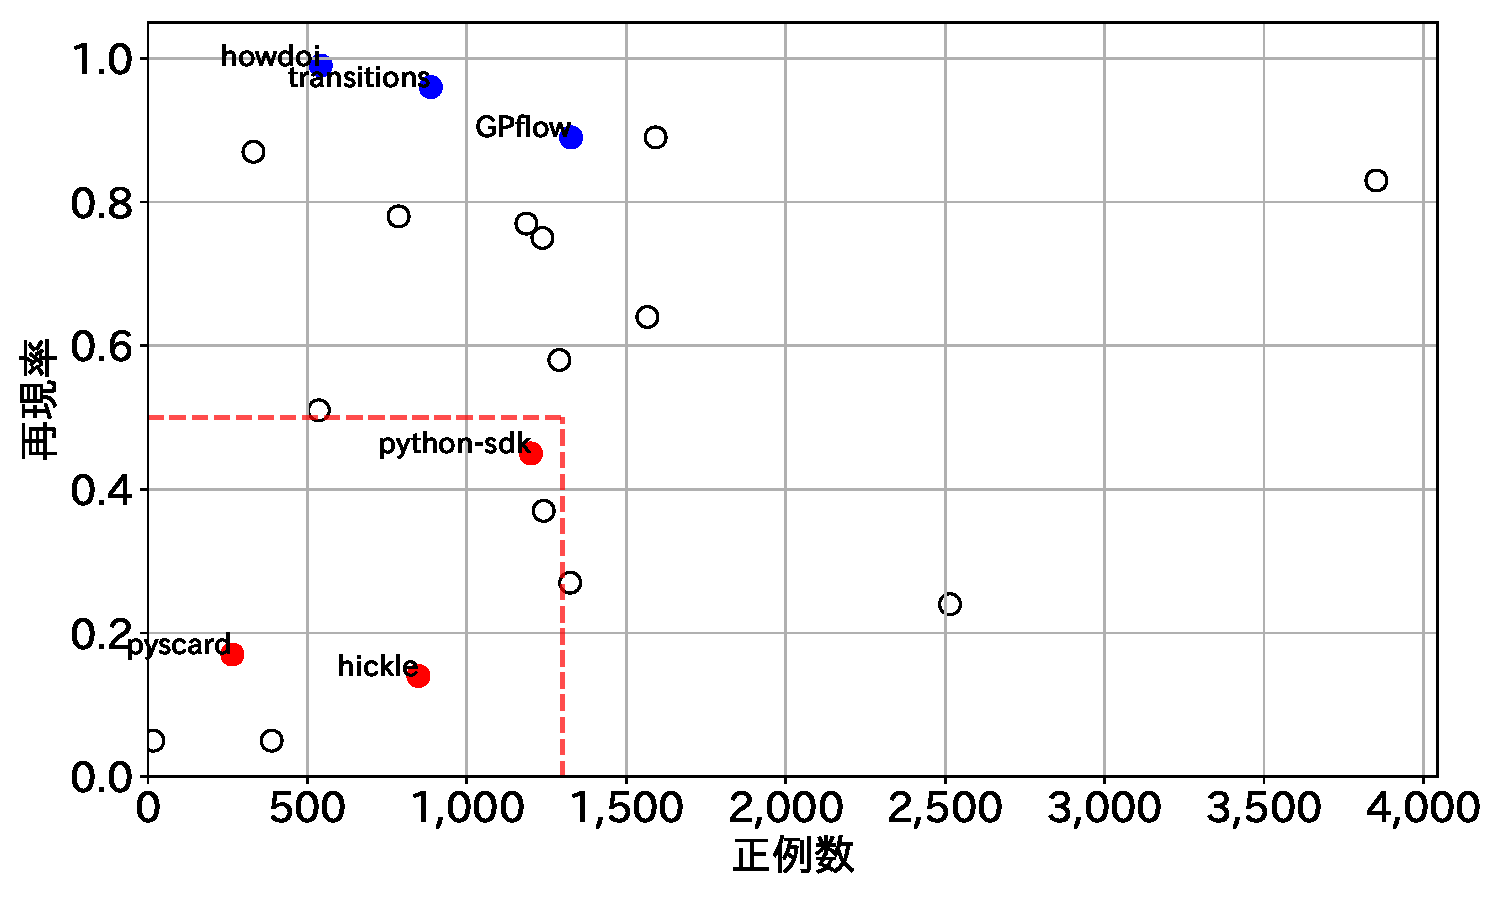
\includegraphics[width=1\linewidth]{fig/sannpuzu.pdf}
	\caption{正例数と単一学習の再現率の散布図}
	\label{fig:scatter_plot_filtered}
\end{figure}
%----------------------

% 結果から,類似プロジェクトの学習データの統合によって,再現率が向上することが示唆された.本節では,この再現率向上が見られるプロジェクトの共通点を分析する.

6プロジェクトは,修正率等が類似する他のプロジェクトの修正履歴を用いて学習データを拡張することで,予測精度が向上した.図\ref{fig:scatter_plot_filtered}は,予測対象プロジェクトの修正履歴に含まれる正例数による再現率の違いを示したグラフである.横軸は各プロジェクトの学習データに含む正例数.縦軸は単一学習の再現率を示す.図\ref{fig:scatter_plot_filtered}には分析対象20プロジェクトの結果を描写している.この中から,選定学習(欠損値補完あり)において複数プロジェクトの学習データを統合して学習した6プロジェクトは,プロットに色とプロジェクト名を付与した.このうち,再現率が10ポイント以上向上したプロジェクトは赤色,それ以外のプロジェクトは青色で示す.

% 4つの手法を比較するため,複数プロジェクトを学習したプロジェクトに着目して分析を進める.単一学習の再現率とデータセットの正例数には,弱い相関(0.35)が見られた.特に,正例数が400以下のプロジェクトでは予測精度がばらついている.

選定学習によって再現率が向上した3プロジェクトは,単一学習の再現率が0.50未満に集中している一方,再現率が低下または同程度だった3プロジェクトは,単一学習の再現率が0.8以上に集中している.したがって,予測対象プロジェクト以外のプロジェクトの修正履歴を統合することで精度向上が期待できるのは,次の2つの共通点を有すると示唆される.
\todo{正例数2500あたりで再現率0.2ぐらいのプロジェクトはなんだろう?正例数が多かったら再現率高いんじゃなかったっけ?}

% この6プロジェクトの分析から,選定学習によって再現率が向上するプロジェクトには,以下の2つの共通点があることが明らかになった.
\begin{enumerate}
    \item データセット内の正例数が1,300以下(図\ref{fig:scatter_plot_filtered}中の赤縦点線).
    \item 単一学習での再現率が0.5以下(図\ref{fig:scatter_plot_filtered}中の赤横点線).
\end{enumerate}

本節では,この2つの共通点におよそ該当する図\ref{fig:scatter_plot_filtered}中の赤点線に囲まれる,再現率が向上した3プロジェクトに加え,学習データを拡張していない5プロジェクトの\todo{XX}を分析する.\todo{図5に対象とするプロジェクト名書いておきたい}
% これらの特徴は,特に選定学習(欠損値補完あり)で学習データを統合したプロジェクトにおいて顕著である.欠損値補完を行わない選定学習では,上記の6プロジェクト以外にも学習データを統合したプロジェクトが存在するため,それらのプロジェクトについても分析を行った.
% 上記の2つの共通点に合致する,または概ね条件を満たしているプロジェクトは,選定学習(欠損値補完あり)で再現率が向上した3プロジェクト以外に,さらに5プロジェクト存在した.


\ihara{学習データを拡張できたのは6プロジェクトで,赤枠で白プロット5プロジェクトは統合していないのでは?次の文章に4プロジェクトは拡張しているようにも読み取れる...}

このうち1プロジェクトは類似プロジェクトが存在せず,単一学習と同様の結果であったため除外した.残る4プロジェクト(serverless-application-model,behave,rtv,datadogpy)について表\ref{table:result1}を用いて分析した結果,behaveプロジェクトを除く3プロジェクトでは,選定学習によって変化がないか,再現率が上昇していることが確認された.


\begin{screen}
総合すると,選定学習によって再現率が向上する上記の2条件を概ね満たすプロジェクトは,選定学習を適用した場合に7プロジェクト中5プロジェクトで再現率の上昇が見られた.
このことから,「データセット内の正例数が1,300以下」および「単一学習での再現率が0.5以下」という2つの条件を満たすことが,複数プロジェクトの学習データを統合することによる恩恵を受けるプロジェクトの有効な特徴であると強く示唆される.
\end{screen}

%%%%%%%%%%%%%%%%%%%%%%%%%%%
\section{考察}\label{chap:consideration}
%%%%%%%%%%%%%%%%%%%%%%%%%%%

\subsection{学習データを統合することによって再現率が向上した要因}

結果として,複数プロジェクトの学習データを統合することで再現率が向上することが示唆された.学習データ統合によって再現率が向上した要因の一つとして,他プロジェクトから正例が補完されたことにより,予測できる正例の範囲が拡大したことが考えられる.

本研究では,学習データのスパース性に対応するため,学習時に正例データへ重みづけを行っている.そのため,補完される正例データが少数であっても,モデルへ大きな影響を与える.これにより,学習データの統合が再現率向上に繋がったと考えられる.

また,全学習で適合率が大幅に低下した要因についても,同様のメカニズムが考えられる.予測対象プロジェクトでは正例としない事象が,他プロジェクトでは正例として扱われていた場合,その数が少量であってもモデルが誤って正例と分類する要因となり,適合率の低下を招いた可能性がある.


\subsection{再現率が向上する条件に一致するが,再現率が低下したプロジェクトの要因}

\begin{figure}[t]
	\centering
        % 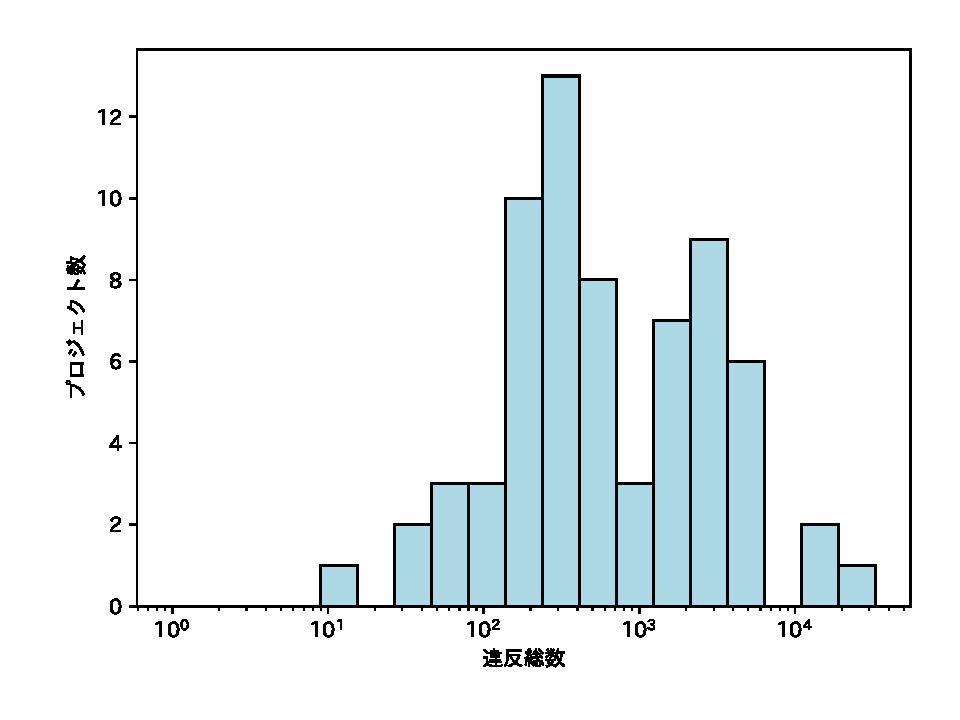
\includegraphics[width=0.25\textwidth, bb=0 0 4 3]{fig/dataset_hist.pdf}
	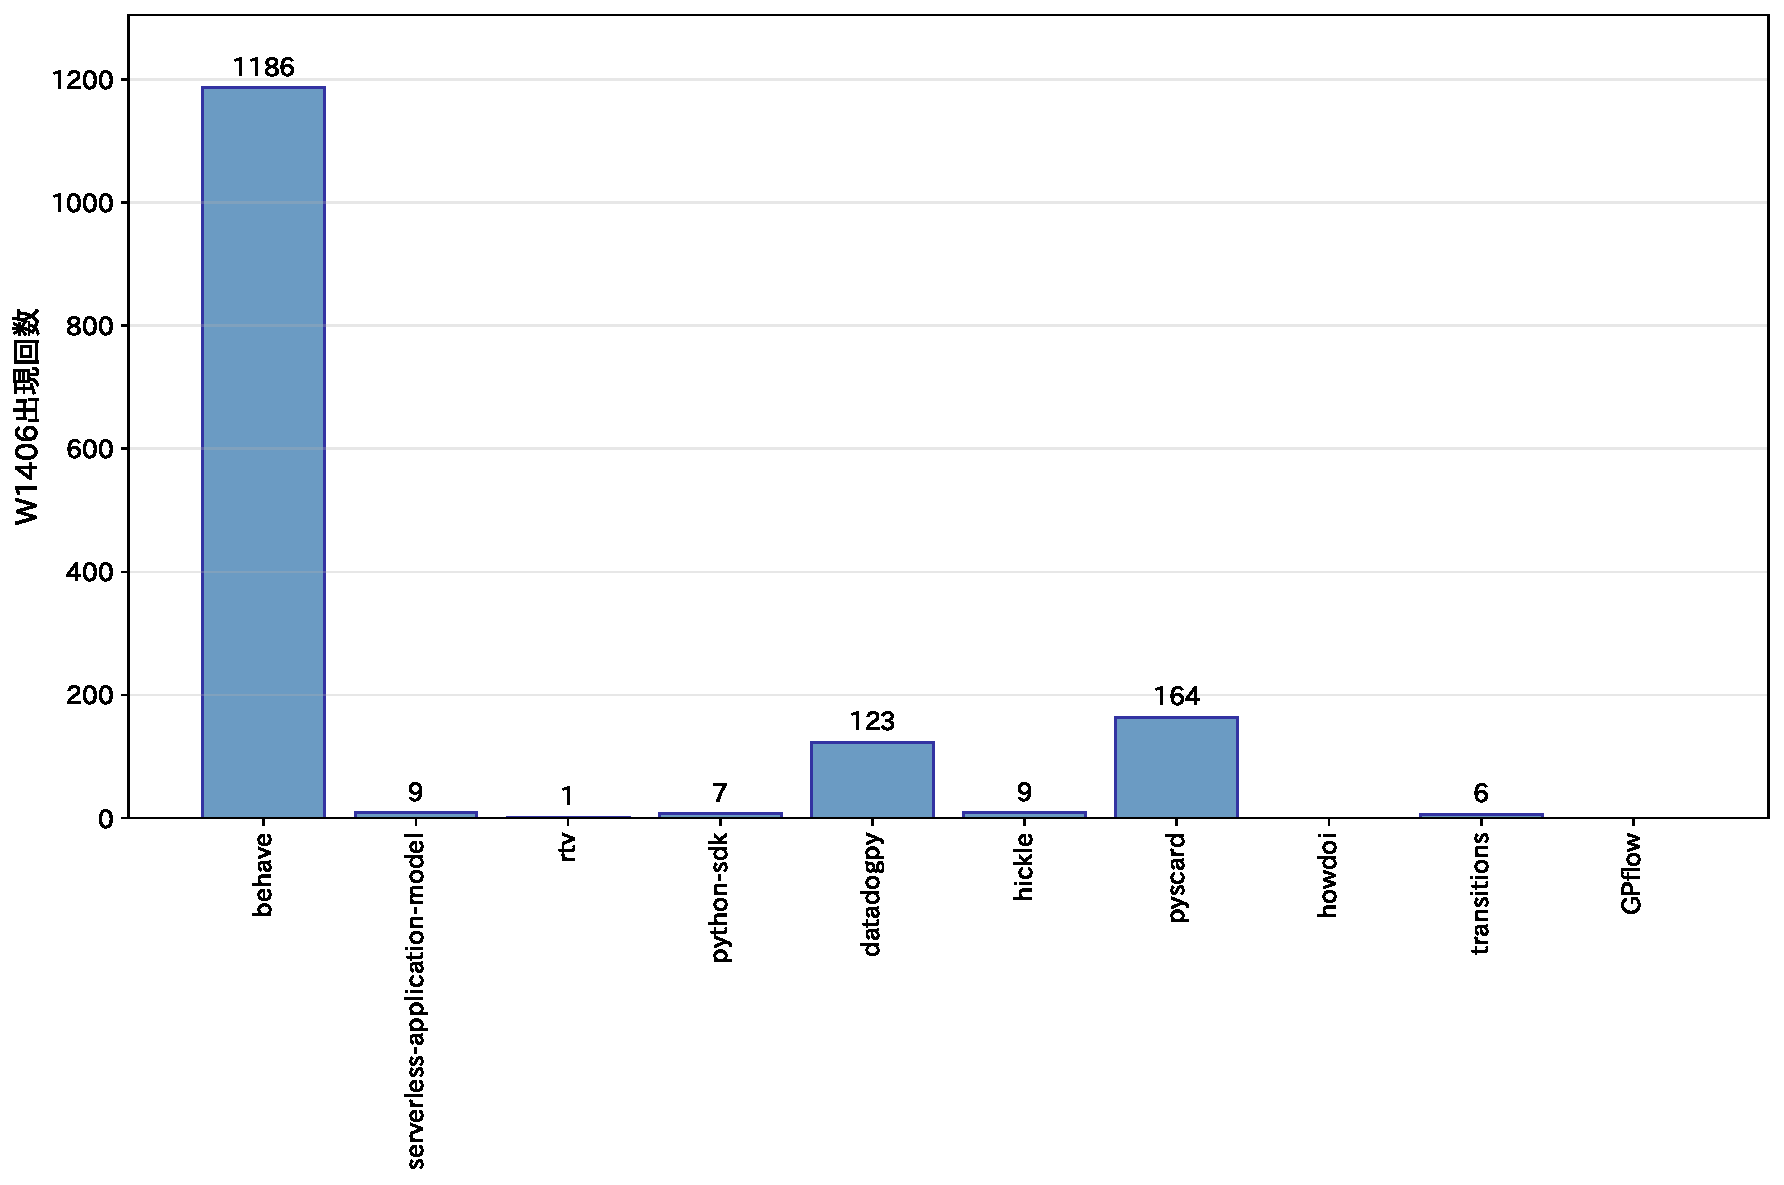
\includegraphics[width=1\linewidth]{fig/w1406_project_comparison.pdf}
	\caption{W1406のプロジェクト別出現頻度}
	\label{fig:w1406}
\end{figure}

behaveプロジェクトは,再現率が向上するプロジェクトの条件を概ね満たしていたにもかかわらず,選定学習によって再現率が13ポイント低下した.本節ではその要因を考察する.

behaveプロジェクトにおけるコーディング規約違反のデータ総数は3,549件であり,そのうち1,186件がW1406という種類のコーディング規約違反であった.これはプロジェクト全体の33\%を占める割合であり,選定学習によって再現率が低下しなかった他の6プロジェクトと比較すると,W1406の出現頻度におけるZスコアは6.95に達する.このことから,W1406がbehaveプロジェクトを象徴するコーディング規約違反であることがわかる.

図\ref{fig:w1406}に示すように,プロジェクトを象徴する特定のコーディング規約が存在する現象は,他のプロジェクトでも同様に見られる.しかし,他のプロジェクトでは,象徴的なコーディング規約の種類が「共通して発生しやすいもの」であるか,または「修正率が低い(正例数が少ないため再現率に影響しにくい)もの」であることが共通している.

一方,behaveプロジェクトを象徴するW1406の修正率は52\%であった.これは,プロジェクト内で当該規約が修正されるか否かの統一された方針が不明確であることを示唆する.さらに,予測精度が向上している他のプロジェクトでは,象徴的なコーディング規約が機械学習モデルの重要度の高い上位10件に含まれる傾向が見られたが,behaveプロジェクトではこの傾向は確認されなかった.

以上の分析から,本研究で提案する選定学習において,他のプロジェクトでは出現頻度の低いコーディング規約が特定のプロジェクト(behave)を象徴する規約となった場合,他のプロジェクトのデータを統合すると,当該プロジェクトを象徴していたコーディング規約の重要度が相対的に低下し,結果として再現率が低下したと考えられる.

%%%%%%%%%%%%%%%%%%%%%%%%%%%
\section{妥当性への脅威}\label{chap:heuristic}
%%%%%%%%%%%%%%%%%%%%%%%%%%%
\subsection{内的妥当性}


目的変数の計測において,規約違反しているコードが修正された場合のみ正例として扱い,削除された場合は,修正されたわけではないため本研究では負例として扱っている.しかし,コーディング規約違反の中には該当部分を削除することによっても解消するものがあるため,本来正例として扱うべきケースを負例として計測してしまっていることがある.
コードの移動に関してもGitHubの仕様上,削除と追加という扱いになるため,コードの移動によってコーディング規約に違反しているコードが削除され不例として計測している可能性がある.
% また,コーディング規約に違反しているコードが,可読性とは関係のない実行速度などの観点からコードが修正された場合でも,違反していたコードが削除された場合は不例として計測してしまっている.


% 本研究で用いた2種類の機械学習アルゴリズム以外にも,より正確な予測を可能にするアルゴリズムが存在する可能性がある.
% それぞれのパラメータの更新回数である,イテレーション回数を10,000に設定したが,データサイズが大きいプロジェクトではモデルが収束しないことが確認された.モデルが収束しない場面も確認されたが,本研究で主に用いた実験環境とは別の環境で,複数回実行した場合でも予測結果に変化はなかったので,モデルが収束しない問題に関しては,本研究の結果に対して大きな影響を与える可能性は低い.


\subsection{外的妥当性}

本研究ではケーススタディとしてPython言語を主な開発言語としたプロジェクト20件の規約違反修正履歴を収集して検証を行った.
また,プロジェクト数をさらに拡張した場合や,対象とするプロジェクトや期間を変更した場合に予測精度が変化することが示唆される.
対象言語をPython以外の言語とした場合予測結果が変化することが示唆される.
しかし,本研究で利用したデータセットは,データ数の平均値が4,465であり,十分なデータ数を確保できているため,データ数を各量することによる予測精度の低下の可能性は低いと考えられる.また,選定学習においては,より類似度の高いプロジェクトを統合できるため,更なる予測精度の向上が見込める.

%%%%%%%%%%%%%%%%%%%%%%%%%%%
\section{おわりに}\label{chap:end}
%%%%%%%%%%%%%%%%%%%%%%%%%%%

本研究では,静的解析ツールによってソースコード中に含まれるコーディング規約違反を検出した結果から,修正すべき違反か否かに分類するタスクにおいて,予測対象プロジェクト以外の開発データも予測モデルの学習に用いた場合の予測結果への影響を調査した.

結果として,予測対象プロジェクト以外の開発データも学習する提案手法によって,検証に使用した20プロジェクトの内,特定の条件を満たす7プロジェクトのうち5プロジェクトで再現率の向上が見られた.再現率が低下したプロジェクトにおいては,発生しているコーディング規約違反の傾向が他プロジェクトと大きく異なる,特殊なデータであった.このことから,条件を満たすプロジェクトであれば,概ね提案手法である選定学習によって再現率の上昇が見込める.

再現率が上昇する理由としては,修正する必要があると判断する正例データが基本的に負例に比べて少ないため,正例データを他プロジェクトからも学習することで,モデルがより多くの修正すべき違反を識別できるようになり,再現率が上昇したと考えられる.

本研究において,選定学習により再現率が向上するプロジェクトの条件が明らかになった.この条件を満たすプロジェクトのデータを拡張して収集し,より類似度の高いプロジェクトのデータを学習することで,単一学習では再現率が低いプロジェクトにおいて,さらなる再現率の向上が見込める.


\begin{biography}
\profile{n}{亀岡 令}{2001年生.2024年和歌山大学システム工学部システム工学科卒業.
同年同大学大学院修士課程入学.}
%
\profile{m}{伊原 彰紀}{2009年奈良先端科学技術大学院大学情報科学研究科博士前期課程修了.2012年同大学博士後期課程修了.2012年同大学情報科学研究科助教.2018年和歌山大学システム工学部講師.博士(工学).ソフトウェア工学,特にオープンソースソフトウェア開発・利用支援の研究に従事.電子情報通信学会,IEEE各会員.}
\end{biography}

\bibliographystyle{ipsjunsrt}
\bibliography{Kameoka}


\end{document}
